\documentclass[a4paper]{report}

% \usepackage[utf8]{inputenc}
% \usepackage[T1]{fontenc}
% \usepackage{textcomp}
\usepackage[english]{babel}
\usepackage{amsmath, amssymb}
\usepackage[separate-uncertainty=true, multi-part-units=single]{siunitx}
\usepackage[]{subfig}
\usepackage[colorlinks=true, anchorcolor=blue, linkcolor=blue, citecolor=blue, bookmarks=false,hyperfootnotes=false]{hyperref}
\usepackage[margin=1in]{geometry}
\usepackage{color,soul}
\usepackage{tabularx}


% figure support
\usepackage{import}
\usepackage{xifthen}
\pdfminorversion=7
\usepackage{pdfpages}
\usepackage{transparent}
\usepackage{physics}
\graphicspath{ {./figures/} }
% \setlength{\parindent}{0pt}
\usepackage{chngcntr}
\usepackage{verbatim}
\usepackage{indentfirst}
\usepackage[most]{tcolorbox}
\usepackage{slashed}
\usepackage{listings}% http://ctan.org/pkg/listings
\usepackage{siunitx}
\DeclareSIUnit\eVperc{\eV\per\clight}
\DeclareSIUnit\clight{\text{\ensuremath{c}}}
\lstset{
  basicstyle=\ttfamily,
  mathescape
}
\numberwithin{equation}{section}
\counterwithin{figure}{section}
\newcommand{\incfig}[1]{%
		\def\svgwidth{\columnwidth}
		\import{./figures/}{#1.pdf_tex}

}

\pdfsuppresswarningpagegroup=1

% for citations / references
\usepackage[style=ieee]{biblatex}
\addbibresource{atlas-report.bib}

\begin{document}

%----------------------------------------------------------------------------------------
%	TITLE PAGE
%----------------------------------------------------------------------------------------
\begin{titlepage} % Suppresses displaying the page number on the title page and the subsequent page counts as page 1
	\newcommand{\HRule}{\rule{\linewidth}{0.5mm}} % Defines a new command for horizontal lines, change thickness here
	
	\center % Centre everything on the page
	%------------------------------------------------
	%	Headings
	%------------------------------------------------
	
	\textsc{\LARGE Rheinische Friedrich-Wilhelms-Universit\"at Bonn }\\[4cm] % Main heading such as the name of your university/college
	
	\textsc{\Large Advanced Laboratory Course}\\[0.5cm] % Major heading such as course name
	
	\textsc{\large Performed on: May 23 - 24, 2022}\\[0.5cm] % Minor heading such as course title

	\textsc{\large Submitted on: June 28, 2022}\\[0.5cm] % Minor heading such as course title
	
	%------------------------------------------------
	%	Title
	%------------------------------------------------
	
	\HRule\\[0.4cm]
	
	{\huge\bfseries E214: ATLAS}\\[0.4cm] % Title of your document
	
	\HRule\\[1.5cm]
	
	%------------------------------------------------
	%	Author(s)
	%------------------------------------------------
	
	\begin{minipage}{0.4\textwidth}
		\begin{flushleft}
			\large
			\textit{Authors}\\
			Keito Watanabe \\
			Paarth Thakkar
		\end{flushleft}
	\end{minipage}
	~
	\begin{minipage}{0.4\textwidth}
		\begin{flushright}
			\large
			\textit{Tutor(s)}\\
			Christina Dimitriadi
		\end{flushright}
	\end{minipage}

	\vspace*{5em}

	\begin{minipage}{0.8\textwidth}
		\begin{centering}
			% \large
			\textbf{Abstract}\\[0.2cm]
            In this experiment, we investigate real and simulated ATLAS data sets and determine the mass of the $W$ boson. We do this by getting familiar with particle reactions at ATLAS using the \texttt{ATLANTIS} program. As a part of the assignment, we studied the \texttt{mystery-035-f.zip} data set and \texttt{ATLASData-Cosmics-M5.zip} data set. After that, we applied calibration to the raw data using the $Z^0$ peak. The calibrated data gave a peak at $91.198 \pm 0.0196$ GeV, which corresponds to the mass of $Z^0$ boson, and we obtain a resolution of $2.342 \pm 0.024$. After applying the calibration to the data, we determined the $W$ boson mass by observing the position of Jacobi peak. We set the QCD background scaling factor to 0.3 and applied cuts of \texttt{el\_etiso} $< 8$ GeV and \texttt{njet} $=0$. Further, we considered uncertainties arising due to systematic errors. Using the gauge curve with half-maximum points from simulated data sets, we obtained a mass of $80.45 \pm 0.10 (\mathrm{stat.}) \: -0.22 \: ^{+0.02}_{-0.03} \: ^{+0.10}_{-0.18} \: (\mathrm{sys.})$ GeV from real ATLAS data. Similarly, we determine the mass of $Z^0$ and we obtain a value of $90.94 \pm 0.20 (\mathrm{stat.}) \: -0.25 \: + 0.02 \: -0.46 \: (\mathrm{sys.})$ GeV. 
            When considering both statistical and systematic errors, we observe that both masses yield values that are within one sigma to the most recent and literature values respectively. 
		\end{centering}
	\end{minipage}
	
	% If you don't want a supervisor, uncomment the two lines below and comment the code above
	%{\large\textit{Author}}\\
	%John \textsc{Smith} % Your name
	
	%------------------------------------------------
	%	Date
	%------------------------------------------------
	
	%\vfill\vfill\vfill % Position the date 3/4 down the remaining page
	% \vfill\vfill
	
	% {\large\today} % Date, change the \today to a set date if you want to be precise
	
	%------------------------------------------------
	%	Logo
	%------------------------------------------------
	
	%\vfill\vfill
	%\includegraphics[width=0.2\textwidth]{placeholder.jpg}\\[1cm] % Include a department/university logo - this will require the graphicx package
	 
	%----------------------------------------------------------------------------------------
	
	% \vfill % Push the date up 1/4 of the remaining page
	
\end{titlepage}

\tableofcontents

\chapter{Introduction} \label{chap:intro}

In this laboratory experiment, we are introduced to the physics of the Large Hadron Collider (LHC). At LHC, proton beams are collided at a center-of-mass energy of $14$ TeV. Such high energies allow us to probe the structure of fundamental particles and study their interactions with high precision. Studying physics at this scale allows us to answer bigger questions, about cosmology, what our universe is composed of and what happened in the events that followed the Big Bang. Further, it could hold answers to physics that has never been observed before, which would further our understanding of the universe. 
This search for answers pushed physicists around the world to build bigger colliders that could reach higher energies. And with each of these came the discoveries of fundamental particles, with the last of them being the Higgs Boson, discovered in the year 2012. 

In this experiment, we start off by getting familiar with \texttt{ATLANTIS}, a program that displays particle reactions graphically. Using \texttt{ATLANTIS} we explored several data sets and got familiar with different kinds of decay channels at LHC. As a part of assignment, we analyzed two different data sets in particular. This is followed by calibration of the raw data, which is done by calibrating the invariant mass distribution of electron positron pair to a well-known Standard Model (SM) parameter, the mass of $Z^0$ boson. After applying the calibration to the data, we measure the mass of the $W$ boson. This is done by observing the position of the Jacobi peak from the electron $p_T$ distribution resulting from $W \rightarrow e\nu$ 
events. We apply the gauge curve to real ATLAS data to determine the mass of $Z^0$ boson to cross check our results. Lastly, we consider systematic errors that arise during the measurements. 

In Chapter \ref{chap:theory}, we briefly go through the important theory behind the SM and the ATLAS detector. In Chapter \ref{chap:prelab}, we provide solutions to the pre-lab questions from the laboratory manual. In Chapter \ref{chap:atlantis}, we use the \texttt{ATLANTIS} program to look at the particle reactions of several data set. Further, we analyze the \texttt{mystery-035-f.zip} data set and \texttt{ATLASData-Cosmics-M5.zip} data set. In Chapter \ref{chap:elec_calib}, we use the well-know parameter of SM, the $Z^0$ mass in order to calibrate our data. This is done by tweaking the energy scaling of different parameters in different regions of its spectrum. In Chapter \ref{chap:wboson}, we use the Jacobi peak to determine the mass of $W$ boson. Further, using simulated data, which considers different masses of $W$ boson, we obtain the parameters for gauge curve, which allows us to obtain the $W$ mass. We cross verify this result by using the curve to determine the mass of $Z^0$ boson. In Appendix \ref{chap:appendix_figs}, we include additional figures for the sake of completeness. In Appendix \ref{chap:appendix_code}, we include the code used for calibration of electrons and macro file used for obtaining half-maximum for each simulated plot. This report closely follows the student lab manual from \cite{labman}. All the constants for SM particles were obtained from \cite{ParticleDataGroup:2020ssz}. All units are in natural units, i.e., $c = \hbar = 1$. 

\chapter{Theory} \label{chap:theory}

\section{The Standard Model}
The Standard Model (SM) is one of the most tested theories in physics. It classifies all the known elementary particles into fermions and bosons and describes three of the four known fundamental forces of nature, strong, weak and electromagnetic force \cite{ParticleDataGroup:2020ssz}. It is a gauge quantum field theory which contains the internal symmetries of the product group, $SU(3) \times SU(2) \times U(1)$. The fermions are spin-1/2 particles and are further classified into quarks and leptons, each with three generations. The bosons are categorized by their spin with gluons, photons, $Z^0$ and $W^{\pm}$ boson having spin 1 and the Higgs boson with spin 0. Apart from the gluons and photons, the other bosons are massive. The elementary particles of the SM are shown in Fig. \ref{fig:sm}.

\begin{figure}[htpb]
    \centering
    \includegraphics[width=0.6\textwidth]{sm.svg.png}
    \caption{The Standard Model particles \cite{wiki:xxx}.}
    \label{fig:sm}
\end{figure}

Despite its huge success, the SM fails at several fronts. It fails to explain matter-antimatter discrepancy, neutrino oscillations, dark matter and hierarchy problem to name a few. In order to test the SM and build a better theoretical framework that tries to answer all of the issues with SM, the Large Hadron Collider (LHC) was built between 1998 and 2008. 

\section{LHC and the ATLAS Experiment} \label{sec:lhc_and_atlas}

\subsection{Large Hadron Collider}

The Large Hadron Collider (LHC) is a circular particle accelerator for proton-proton collisions, located at the European Organization 
for Nuclear Research (CERN) at Geneva, Switzerland. Within the accelerator, two proton beams, accelerated and guided by superconducting 
cavities and electromagnets respectively, traverse in opposite directions propagating close to the speed of light. These beams then 
collide at four different interaction points with a center-of-mass energy of up to $E_{\mathrm{CM}} = \SI{14}{\tera\electronvolt}$,
 corresponding to the following experiments: ALICE, LHCb, CMS, and ATLAS. \par

In our laboratory experiment, we work with the simulated and real data obtained from the ATLAS detector from proton-proton collisions at center-of-mass
energies at $\SI{14}{\tera\electronvolt}$, and as such we will focus on the ATLAS detector in this report.

\subsection{The ATLAS Detector}

The ATLAS detector (\textbf{A} \textbf{T}oroidal \textbf{L}HC \textbf{A}pparatu\textbf{S}) is the largest detector placed at the LHC. It is 46m long, 25m high, 
and weighs approximately 7000 tons. The massive size of the detector allows coverage of almost all solid angles. The ATLAS detector is a multi-layed structure, 
consisting of different detector components constructed to detect the many 
different particles that emerge from the final products of the collision. See Fig. \ref{fig:atlas_detector} for a schematic of the ATLAS detector. The detector components can largely 
be divided into three regions: the Inner Detector, Calorimeter, and the Muon System. 

\begin{figure}[htpb]
    \centering
    \includegraphics[width=0.8\textwidth]{ATLASDetector.jpg}
    \caption{The schematic of the ATLAS detector. Obtained from Ref. \cite{ATLASFactSheet}.}
    \label{fig:atlas_detector}
\end{figure}

\subsubsection{(a) Inner Detector}

The inner detector is the closest detector from the interaction point. To properly reconstruct the primary vertex, the detectors in this region are very 
sensitive. The inner detector, along with the solenoid surrounding it, allows measurements of the direction, momentum, and electrical charge of the 
produced particles in the proton-proton collision. The inner detector can subsequently be separated into four parts. \\ 

\noindent \textit{Pixel Detector} \\ \\
The pixel detector is located most closest to the interaction point with a radial distance of $5 - 15$cm to the proton beam. The detector processes signals of 
over 80 million pixels, thus having the most readout channels out of all the detector components. This allows sensitive measurements on the charged particle 
trajectory (hits) as well as reconstruction of the primary vertex. It also helps in reconstruction of secondary trajectories, which occur in decay of b-quark 
hadrons. \\ 

\noindent \textit{Semi-Conductor Tracker (SCT)} \\ \\ 
This component is placed in between the pixel detector and the Transition Radiation Tracker (TRT). It operates similarly to the pixel detector, but 
silicon strips with length $\SI{80}{\micro\metre}$ are used instead of pixels. These silicon strips allow measurements of the position of the 
charged particles to an accuracy of $\SI{17}{\micro\metre}$ per layer. The area is also much larger than the pixel detector, making it an important component 
of the inner detector \cite{ATLASFactSheet}. \\ 

\noindent \textit{Transition Radiation Tracker (TRT)} \\ \\ 
This component is placed at the outermost part of the inner detector. This detector consists of both a straw tracker and a transition radiation detector. 
The noble gas contained within each straw ionizes and produces a signal in the wire when a charged particle passes through it. The signal is further enhanced 
by transition radiations that occur due to the materials contained between the straws. This tracker helps to distinguish the type of charged particle that
flew into the detector, for example whether if it is an electron or a pion \cite{ATLASFactSheet}. \\ 

\noindent \textit{Solenoid} \\ \\ 
The inner solenoid is a superconducting magnet surrounding the inner detector. It provides the inner detector with a solenoidal magnetic field strength of 
$\SI{2}{\tesla}$, allowing the charged particles to bend due to the Lorentz force. This allows one to distinguish the electric charge of the particle 
as well as measure the momentum $p$ through the radius of curvature of the particle. This can be shown by equating the Lorentz force to the 
centripetal force:
\begin{equation}
	|\vec{F_L}| = |\vec{F_C}| \implies evB = \frac{mv^2}{R} \implies R = \frac{mv}{eB} = \frac{p}{eB}
	\label{eq:rad_curvature}
\end{equation}
where $\vec{v} \perp \vec{B}$ from the detector geometry. We further observe that positively and negatively charged particles will have 
opposite radius of curvatures. As neutral particles such as photons or neutrons 
have no electric charge, they show no curvature when they traverse through the inner detector. 

\subsubsection{(b) Calorimeter}

The calorimeter, placed outside the solenoid, measures the total energy of the particles. These particles are often entirely stopped 
within the calorimeter, forcing all of their energies to be deposited in the detector. There are two types of calorimeters used. \\

\noindent \textit{Presampler} \\ \\
Before the calorimeters, a presampler is placed to support measurement of electromagnetic showers. Specifically, it helps to distinguish between single photons a
and photons from $\pi^0$ decays. \\ 

\noindent \textit{Electromagnetic Calorimeter (ECAL)}\\ \\
The electromagnetic calorimeter (ECAL) absorbs the energies of particles that interact electromagnetically, that is, those with an electric charge as well as the photon. 
It consists of alternating layers of iron and liquid argon, acting as the absorber and the ionization chamber respectively. The ECAL is folded similarly to 
an accordion such that it has an angle of $\SI{45}{\degree}$ with respect to the charged particle trajectories.  \par 

In the ECAL, electromagnetic showers, that is, a cascade of interactions between photons, electrons, and positrons, are produced and measured. At the relevant energy 
regime, photons and electrons (and positrons) interact with matter most commonly via Compton scattering, pair production, or bremsstrahlung. 
These three interactions occur interchangeably, producing subsequent electrons and photons. This leads to a cascade of such particles, which is known as an 
electromagnetic shower. The number of particles produced in this shower is proportional to the primary energy. 
The longitudinal extension is described by its radiation length $X_0$, defined such that after one radiation length an electron only retains 
$1 / e$ of its initial energy. These radiation lengths in solids are typically of order cm. \par 

As muons have a higher mass, they do not undergo bremsstrahlung and as such not detected in the ECAL\footnote{Muons with energies TeV or higher do lose their energy via 
bremsstrahlung significantly and show signature in the ECAL before leaving the detector.}. As such, a separate system is constructed to detect muons, which will be mentioned 
in the subsequent subsection. \\

\noindent \textit{Hadronic Calorimeter (HCAL)} \\ \\
The hadronic calorimeter (HCAL) are used to produce and detect hadronic showers, that is, cascades produced by hadrons (mostly pions and kaons). 
The HCAL operates in a similar fashion to the ECAL, however, the size of the HCAL is much larger, ensuring that the hadrons are absorbed completely. The shower layers 
consist of iron, and to detect such particles liquid-argon chambers and scintillation tiles are used. \par 

The hadronic showers generated in the HCAL are produced by inelastic interaction between the hadron and the nuclei in the material. These hadrons interact strongly, 
producing numerous hadrons and nuclei remnants, producing subsequent hadrons. This causes an avalanche of reactions, constructing a hadronic shower. Similar to 
electromagnetic showers, the longitudinal extension of the hadronic shower is estimated by its hadronic interaction length $\lambda$. The interaction length is 
defined such that after one interaction length, the number of hadrons that did not yet take part in the strong interaction decreases to $1 / e$. The interaction 
length is often much larger than the radiation length. 

\subsubsection{(c) The Muon System}

As previously mentioned, muons do not emit bremsstrahlung and thus are not absorbed by the ECAL. Thus a separate system is necessary to measure the muon trajectory 
and momentum. In the muon system, tracking chambers that fill up to half of the detector's volume is placed outside the calorimeters. The number of hits are then 
measured, allowing for measurements in the muon's position. Furthermore, large superconducting toroids are placed outside the tracking chambers with a magnetic 
field strength of $\SI{4}{\tesla}$, allowing measurements of the muon's momentum as well. \\

\subsection{Interaction of Particles in Detectors}

As mentioned in the previous section, different detector components allows measurements of different type of particles. In this 
section, we highlight the signature of each particle in the detector. Fig. \ref{fig:detector_signatures} shows a schematic of all such signatures. 

\begin{figure}[htpb]
    \centering
    \includegraphics[width=0.6\textwidth]{detector_signatures.png}
    \caption{Signatures of different particles observed in the ATLAS detector. The electromagnetic and hadronic cascades can be seen from the ECAL and HCAL 
	respectively. Obtained from Ref. \cite{Gerber2019}. }
    \label{fig:detector_signatures}
\end{figure}
\bigbreak
\noindent \textit{Electrons and Positrons} \\ 

Electrons and positrons are mostly highly relativistic due to its smaller mass. They are electrically charged and thus bend when 
hits are measured in the inner detector. As they undergo bremsstrahlung and Compton scattering, they are readily absorbed in the ECAL, 
generating an electromagnetic cascade. \\

\noindent \textit{Photons} \\

Photons are electrically neutral and are highly energetic with energies $> \SI{1}{\giga\electronvolt}$, so they do not show any hits
 in the inner detector. However, they undergo pair production and Compton scattering and are thus absorbed in the ECAL. Thus photons 
 also produce an electromagnetic cascade. \\

 \noindent \textit{Hadrons} \\

 Hadrons which are electrically charged ($\pi^\pm, K^\pm, p, \bar{p}$ etc) bend when their hits are observed as with $e^-, e^+$, 
but do not leave any signature in the ECAL as they are much heavier than electrons and positrons. They are, however, absorbed in the HCAL, 
producing a hadronic cascade. \par 

Hadrons which are electrically neutral, such as neutrons do not leave any hits in the inner detector nor do they produce 
any electromagnetic cascades. As they interact strongly, they produce hadronic cascades in the HCAL, making the curvature in the trajectories
the only way to distinguish between electrically charged and neutral hadrons. Neutral pions are an exception to this as they primarily decay 
into photon pairs, which are subsequently observed in the ECAL. \par 

Hadrons containing b quarks have an extremely long lifetime as the b quark itself has a long lifetime. They most often decay inside the beam pipe, located 
outside the detector system itself. As the decay vertex is far away enough from the primary vertex, suitable reconstruction methods can be used to identify the 
B hadrons. This is done by b-jet tagging, where the innermost detector is used to identify the jets from the b quarks. \\

\noindent \textit{Muons} \\

Muons are charged leptons and thus their trajectories bend in the inner detector. Due to their high mass, however, they do not emit bremsstrahlung and thus 
do not leave any signature in both ECAL and HCAL. They are separately measured by the tracking detectors placed outside the calorimeters, where the curvature 
of the trajectory can be observed due to additional magnetic field placed. \\

\noindent \textit{Tau} \\

Tau leptons ($\tau^\pm$) are much heavier than muons ($m_\tau \approx \SI{1}{\giga\electronvolt}$) and their range in matter is limited do millimeters 
as they have a short lifetime. They most commonly decay weakly into hadrons ($\tau^- \rightarrow \mathrm{hadrons} + \nu_\tau$), which can be identified in the detector as collimated ``mini jets''. \\

\noindent \textit{Top Quark} \\

The top quark is the only quark which decays before it can form jets due to its heavy mass of approximately $\SI{170}{\giga\electronvolt}$. They 
primarily decay weakly via $t \rightarrow W^+ b$, i.e. to a b-quark. The top quarks can be identified by the decay products of the $W$ boson and the 
jets from the b-quark, i.e. with three jets or jets with a $l\nu_l$ pair. \\

\noindent \textit{Neutrinos} \\

Neutrinos only interact weakly and thus direct detection of single neutrinos within this detector is not possible. However, neutrinos with a high enough 
transverse momentum are detected indirectly by using conservation laws. This will be further elaborated in Sec. \ref{sec:gauge_bosons}.

\subsection{Coordinate System} 

In Cartesian coordinates, we set the axes such that the origin is placed at the collision point. 
The $z$ axis is defined to be aligned with the beam axis. The $x$ axis is defined such that it 
points towards the center of the LHC ring. The $y$ axis is defined to be perpendicular to the beam axis. 
\par

From this, we can defined relevant quantities that are frequently used to describe the detector coordinates:
\begin{itemize}
	\item Radial distance to z-axis $\rho = \sqrt{x^2 + y^2}$ 
	\item Azimuthal angle $\phi$, defined from the x-axis 
	\item Polar angle $\theta$. The angle is defined such that $\theta = 0$ is aligned with the xz-plane and $\theta = \pi / 2$ is 
			aligned with the y-axis. 
\end{itemize}
A schematic of the coordinate system with the above relevant quantities is shown in Fig. \ref{fig:atlas_coord}.

\begin{figure*}[htpb]
    \centering
    \includegraphics[width=0.7\textwidth]{atlas_coords.png}
    \caption{Schematic of the coordinate system defined for the ATLAS detector. The radial distance to the z-axis $\rho$, 
	azimuthal angle $\phi$ and polar angle $\theta$ is also shown. Image based on Ref. \cite{Rivera2018}.}
    \label{fig:atlas_coord}
\end{figure*}

We also define the pseudorapidity $\eta$ as such: 
\begin{equation}
	\eta = -\ln \tan (\frac{\theta}{2})
\end{equation}
where $\theta$ is the polar angle. The pseudorapidity is defined such that $\eta = \pm\infty$ is defined in the direction of the 
$\pm \hat{z}$ axis respectively. Fig. \ref{fig:pseudorap} shows how the pseudorapidity and polar angle are related. The ATLAS 
detector detects leptons in $|\eta| < 2.5$ and jets in $|\eta| < 5$.
Using the pseudorapidity is especially useful for the ATLAS experiment as the final products from proton-proton collisions increases 
strongly in the forward direction (near the beam axis). 

\begin{figure*}[htpb]
    \centering
    \includegraphics[width=0.5\textwidth]{pseudorapidity.pdf}
    \caption{The pseudorapidity and its relation to the polar angle. The values from the y-axis to the +z-axis is shown. 
	Obtained from Ref. \cite{Izaak2017}.}
    \label{fig:pseudorap}
\end{figure*}


\section{The Heavy Gauge Bosons} \label{sec:gauge_bosons}

The $W^{\pm}$ and $Z^0$ are massive bosons which are responsible for the weak forces. The electromagnetic and the weak interactions are unified in the SM to give the electroweak force. The electromagnetic force arises due to $U(1)_{Y}$ ($Y$ is hypercharge) gauge symmetry and the weak force arises due to $SU(2)_L$ ($L$ is left-handed chiral) gauge symmetry. After Spontaneous Symmetry Breaking (SSB), the $W^{\pm}$ and $Z^0$ gain mass while the photon continues to be massless. In this experiment, our aim to is learn the methods of measuring the mass of the $W$ boson. Some important vertices of weak interaction are shown in Fig. \ref{fig:weak_int}.

\begin{figure*}[htb!]
	\centering
	\subfloat[Fermion anti-fermion going to $Z^0$ boson or a virtual photon to give lepton anti-lepton pair. \label{subfig:ztoll}]{{\includegraphics[width=0.47\columnwidth]{feynman(1)}}}
	\quad
	\centering
	\subfloat[Fermion anti-fermion going to $W^{\pm}$ to give lepton (anti-lepton) and anti-neutrino (neutrino). This process is the weak Drell-Yan process. \label{subfig:wtolnu}]{{\includegraphics[width=0.47\columnwidth]{feynman(2)}}}
	\quad
	\centering
	\subfloat[Fermion anti-fermion going to $Z^0$ boson or a virtual photon to give $W^{\pm}$ pair. \label{subfig:ztoww}]{{\includegraphics[width=0.47\columnwidth]{feynman(3)}}}
	\caption{Important weak interactions at LHC. Here $f$ stands for fermion and $l$ for leptons.}
	\label{fig:weak_int}
\end{figure*}

The mass of the $Z^0$ boson has been measured with high precision at the LEP accelerator in the year 2006 \cite{ALEPH:2005ab}. Its mass was found to be $91.1876 \pm 0.0021$ GeV. Since the $Z^0$ boson decaying to leptons (as shown in Fig. \ref{subfig:ztoll}) gives the cleanest signal to reconstruct its invariant mass, these events are usually studied. However, in the case of $W$ boson, which decay to $W \rightarrow e\nu_e$ or $W \rightarrow \mu \nu_{\mu}$, the invariant cannot be reconstructed directly. This is because neutrinos interact weakly and are not detected. This makes measuring the mass of the $W$ boson a challenge and it is also one of the less known parameters of the SM. As of writing this report, a high precision measurement by the CDF collaboration of $W$ boson mass was made in April, giving a value of $80.433 \pm 0.009 \ \text{GeV}$ \cite{CDF:2022hxs}. This result has a 7$\sigma$ deviation from the SM prediction, suggesting inaccuracies in the calculations or possibility of new physics. Before this, the most precise measurement was made in 2018 and found to be $80.379 \pm 0.012 \ \text{GeV}$ \cite{PhysRevD.98.030001}. 

There are two notable ways to measure the mass of the $W$ boson. The first utilizes the variable $\text{M}_\text{T}$, which is defined as

\begin{equation}
\mathrm{M_T} = \sqrt{2 p_{T_e} p_{T_{\nu}} (1 - \cos(\phi_e - \phi_{\nu}))},
\end{equation}
where $p_{T_e}$ and $p_{T_{\nu}}$ are the transverse momentum of the electron and neutrino respectively, $\phi_e$ and $\phi_{\nu}$ are the azimuthal angles. If we consider the mass of the electron to be zero, $\mathrm{M_T}$ is equal to $W$ mass. The distribution of $\mathrm{M_T}$ gives us a Jacobi peak at the W mass. The advantage of using this method is that the transverse of momentum of the $W$ boson does not significantly affect the position of the peak. The disadvantage is the use of $p_{T_{\nu}}$, which as mentioned before, cannot be measured directly. Hence, it must be approximated using $\slashed{E}_T$, which is missing transverse momentum, given by

\begin{equation}
	\vec{\slashed{E}_T}	= - \sum_{i} E^i \sin \theta_i \vec{n}_{i, \perp},
\end{equation}
where $E^i$ is the energy of the $i$-th entry in the calorimeter, $\theta_i$ is the polar angle of the entry and $\vec{n}_{i, \perp}$ is the unit vector pointing towards energy entry in the x-y plane. Which means, that in order to measure $\mathrm{M_T}$ accurately, $\slashed{E}_T$ has to be well calibrated. 

The second method to measure the $W$ mass is by studying the transverse momentum spectrum of the leptons using

\begin{equation}
	\frac{d \sigma}{d p_T} = \frac{d \sigma}{d \cos \theta ^*} \left| \frac{d p_T}{d \cos \theta ^*} \right| ^{-1} = \frac{d \sigma}{d \cos \theta ^*} \frac{2p_T}{M_W} \frac{1}{\sqrt{1/4 \ M_W^2 - p_T^2}}.
\end{equation}
This gives a Jacobi peak as shown in Fig. \ref{fig:jacobi}. The peak is at half of $W$ mass, therefore, one can measure this peak in order to deduce the $W$ mass. However, the figure shows the ideal case, in which the $W$ boson does not have an initial transverse momentum. As shown in the same figure, if $W$ has an initial momentum, there is a spread in the distribution and a shift in the Jacobi peak. Other factors that can increase the spread are the resolution of the detector and $W$-decay width. However, the advantage of using this method is that it does not require the complicated calibration of $\slashed{E}_T$. In this experiment we use this method. An interesting side note, the recent high precision measurement from 2022 used the first method to measure the $W$ mass \cite{CDF:2022hxs}.


\begin{figure}[htpb]
    \centering
    \includegraphics[width=0.6\textwidth]{jacobi}
    \caption{$p_T$ spectrum of leptons from the $W \rightarrow l \nu$ decay. We see a Jacobi peak at half the mass of $W$ boson \cite{jacobi}.}
    \label{fig:jacobi}
\end{figure}


\chapter{Pre-lab Questions} \label{chap:prelab}

\section{Part 2: Calibration of Electrons}

\noindent 1. Which value does the momentum of an electron have in the decay of a $Z^0$ boson $Z^0 \rightarrow e^+ + e^-$, if the $Z^0$ is at rest? 
\bigbreak
\noindent \underline{Solution}: \\
\noindent Given that the $Z^0$ boson is at rest, $\vec{p}_Z = 0 \implies E_Z^2 = \vec{p}_Z^2 + m_Z^2 = m_Z^2$ so that $E_Z = m_Z$. This implies that the 4-momentum of the $Z^0$-boson is $p_Z = (m_Z, \vec{0})$. 
\noindent Now by conservation of 4-momentum, we know that $p_Z = p_{e^+} + p_{e^-} \implies p_{e^+} = p_Z - p_{e^-}$. 

\noindent Now taking the dot product of $p_{e^+}$, we have that:
$$
p_{e^+} \cdot p_{e^+} = m_e^2 = (p_Z - p_{e^-}) \cdot (p_Z - p_{e^-}) = m_Z^2 + m_e^2 - 2 p_Z \cdot p_{e^-} = m_Z^2 + m_e^2 - 2m_Z E_e
$$
$$
\implies m_Z = 2E_e => E_e = \frac{m_Z}{2}
$$
\noindent where the property $(p \cdot p) = E^2 - \vec{p}^2 = m^2$ was used. 

\noindent To then determine the momentum of the electron, we use the energy-momentum relation again:
$$E_e^2 = \vec{p}_e^2 + m_e^2 \implies |\vec{p}_e| = \sqrt{E_e^2 - m_e^2} = \sqrt{\left(\frac{m_Z}{2}\right)^2- m_e^2}$$
$$\implies |\vec{p}_e| = \sqrt{\left(\frac{91.18 \text{GeV} }{2}\right)^2 - (5.11 \times 10^{-4} \text{GeV})^2} \approx 45.59 \text{GeV}$$

\noindent where the mass of the electron was neglected. 

\noindent Thus the momentum of the electron from a $Z^0$ boson decay at rest is $|\vec{p}_e| = 45.59 \text{GeV}$. 

\bigbreak

\noindent 2. How large is the momentum of tau leptons in the reaction $e^+ + e^- \rightarrow \tau^+ + \tau^-$, if the reaction takes place in the center-of-mass system (center-of-mass energy = 5 GeV)?
\bigbreak
\noindent \underline{Solution}: \\
\noindent We know that the mass of the tau lepton is $m_\tau = 1.776$ GeV. Given that the CoM energy is $\sqrt{s} = 5$ GeV, by conservation of energy we have that:
$$s = (2 E_e)^2 = (2 E_\tau)^2 = 4 (\vec{p}_\tau^2 + m_\tau^2) \implies |\vec{p}_\tau| = \sqrt{\frac{s}{4} - m_\tau^2}$$

$$
\implies |\vec{p}_\tau| = \sqrt{\frac{(5 \text{GeV})^2}{4} - (1.776 \text{GeV})^2} = 1.7595 \text{GeV}
$$

\section{Part 3.1: W-Boson Measurement}

\noindent 1. As before, the analysis is based on ROOT trees. One of the tree variables is $\texttt{ptw -}$  the estimated transverse momentum of the $W$ boson candidate. This variable can be constructed from the other tree variables. Please think about how this could be done. The tree variables are listed in section B.
\bigbreak
\noindent \underline{Solution}: \\
\noindent Given that the weak interaction is described by $W \rightarrow l + \bar{\nu}_l$, we can calculate the transverse momentum of the $W$ boson from the transverse momentum of $l$ and $\bar{\nu}_l$.  The formula to evaluate this is:
$$p_{T_W} = \sqrt{p_{T_l}^2 + p_{T_\nu}^2}  $$
which is derived from the conservation of 3-momentum.

\noindent This is defined in ROOT as $\texttt{el\_pt} \ \text{and} \ \texttt{etmis}$, so that the transverse momentum of the $W$ boson candidate can be calculated as such: $\sqrt{\texttt{el\_{pt}}^2 + \texttt{etmis}^2}$.

\bigbreak 

\noindent 2.  When fitting measurements to a linear function, the two parameters of a best fit straight line are y-intercept and slope. The errors on these parameters are typically correlated. Using these parameters for the error analysis will require a treatment that takes correlations into account. For example the simplest form of Gauss’ error propagation law requires that the errors are uncorrelated. Please look up the correct form of the Gauss error propagation law in the presence of correlations. You will need that for the final error on the W mass. On the other hand, is it possible to minimize correlations by choosing an appropriate coordinate system?
\bigbreak
\noindent \underline{Solution}: \\
\noindent The Gauss error propagation law in the presence of correlations is given as such:
$$
	\sigma_f ^2 = \left( \frac{df}{dx} \right)^2 \sigma_x^2 + \left( \frac{df}{dy} \right)^2 \sigma_y^2 + 2 \left( \frac{df}{dx} \right) \left( \frac{df}{dy} \right) \rho_{xy} \sigma_{x} \sigma_y $$
	
\noindent where $\rho_{xy}$ is the correlation coefficient which yields zero for uncorrelated errors. The correlation matrix is then defined with the variance $\sigma_x^2, \sigma_y^2$ in its diagonals with the correlations $\rho_{xy} \sigma_x \sigma_y$ in the off-diagonal components.

\noindent To minimize correlations, we can convert to an appropriate coordinate system in which the correlation matrix becomes diagonal. This will allow the cross terms to vanish.

\section{Part 3.2: New Physics}

\noindent 1. What is the minimum invariant 4-lepton-mass, when the four leptons originate from a $Z^0$ pair? Why do you find 4-lepton-events with invariant mass beneath this threshold?
\bigbreak
\noindent \underline{Solution}: \\
\noindent In theory, the minimum invariant mass of the each lepton should be $m_Z / 2$. In addition to the lowest order Feynman diagrams, there are two higher order diagrams where the photon is radiated by initial-state quarks, called Initial State Radiation (ISR), due to which there is a shift in the energy of the ingoing particles, leading to a distortion in the shape of the $Z^0$ resonance curve. Therefore, the effect of ISR is reduce the effective centre-of-mass energy of the ingoing particles, which leads to some fraction of $Z^0$ boson invariant mass to be beneath this threshold. 
Another possible reason can be that in the case of more than one $Z^0$ boson, the other $Z^0$ boson will not be on-shell due to kinematic reasons. Due to this, we get one $Z^0$ boson and another virtual Z* boson. Hence, the mass of the 4 leptons, would be below the threshold. 

\bigbreak

\noindent 2. Consider a Higgs boson which decays into two $Z^0$ bosons. How does the distribution of the 4-lepton-invariant-mass look like?
\bigbreak
\noindent \underline{Solution}: \\
\noindent The distribution will follow a Voigt function peaked at ~125 GeV (Fig. \ref{fig:higgs-decay}).

\begin{figure}[htpb]
    \centering
    \includegraphics[width=0.6\textwidth]{higgs-decay}
    \caption{ATLAS four lepton invariant mass measurement showing evidence for the Higgs boson \cite{ATLAS:2020wny}.}
    \label{fig:higgs-decay}
\end{figure}

\bigbreak

\noindent 3. Assume you have an ideal detector. What is the typical $\slashed{E}_T$ if a $Z^0$ pair has been produced and both $Z^0$ decay into electron or muon pairs? What $\slashed{E}_T$ will you expect when you have a real detector?
\bigbreak
\noindent \underline{Solution}: \\
\noindent In an ideal case, the expected $\slashed{E}_T$ is 0. In the case of real detector, $\slashed{E}_T$ will be non-zero due to inefficiencies in the detector and reconstruction algorithms. Further, not all muons and electrons will be detected. Or, one of the leptons could be extremely soft and not be detected at all. 

\bigbreak

\noindent 4. The Branching ratio of $t \rightarrow W b$ is almost 100\%. If you have a top anti-top pair in an event, both particles decay instantly via $t \rightarrow W b$. If both $W$ bosons each decay leptonically ($W \rightarrow l \nu$), one finds two leptons in the event. What could explain the occurence of four leptons in a $t \bar{t}$ event?
\bigbreak
\noindent \underline{Solution}: \\
\begin{itemize}
	\item One of the leptons radiates a photon/Z* boson which gives lepton-antilepton pair, $l \rightarrow l + \gamma \rightarrow l + l^+ + l^-$.
	\item b-quark can decay semi-leptonically, giving us hadrons plus a lepton (Fig. \ref{fig:bdecay}).
\end{itemize}

\begin{figure}[htpb]
    \centering
    \includegraphics[width=0.6\textwidth]{bdecay}
    \caption{Top and b-quark decay process \cite{labman}.}
    \label{fig:bdecay}
\end{figure}

\chapter{ATLANTIS} \label{chap:atlantis}

In this part of the lab, we get familiar with the program \texttt{ATLANTIS}, which displays particle reactions in the ATLAS detector graphically. 
From this program, one can easily retrieve relevant quantities such as the particle's transverse momentum, azimuthal angle and pseudorapidity
from the given datasets. 
Before looking at the assignments for this part, we first become acquainted with all the data sets. We present our observations below. 

\section{Electron Dataset}

In this dataset, we observe the signature of a single electron in the detector. Fig. \ref{fig:single_e} shows the output from ATLANTIS for Event 7 in the 
dataset. In each figure shown in this section, the upper left figure shows the xy projection of the 
event. The upper right top shows a zoomed-in xy projection at the inner detector. The upper right lower figure shows the $\rho$z 
projection, and the lower figure again shows the zoomed-in $\rho$z projection at the inner detector and calorimeters. The blue line
 are the reconstructed tracks and the yellow boxes are the energy depositions in the calorimeters. Finally, the red dashed line 
 indicates the $\slashed{E}_T$ obtained from kinematical calculations.

\begin{figure}[htpb]
    \centering
    \includegraphics[width=0.6\textwidth]{electron_event7.eps}
    \caption{Event name: \texttt{singlepart\_electron-1\_0\_00007\_f}, Event: 7. }
    \label{fig:single_e}
\end{figure}

From this event, we observe that the electron, contrary to the its electric charge, traverses without bending. This is most likely
due to the high momentum of the electron ($p_T = \SI{-6.03 \pm 0.097}{\giga\electronvolt}$), increasing the radius of curvature as shown in Eq. \ref{eq:rad_curvature}. We also observe 
signatures in the ECAL, indicating that the electron has produced an electromagnetic cascade, and has thus been absorbed completely. 
We also observe signatures in the HCAL, which are attributed to the background of the event. The $\slashed{E}_T$ shown in the 
figure also result from background processes as $\slashed{E}_T \approx \SI{61}{\giga\electronvolt}$, which is much larger than the 
electron momentum. \par 

\section{Muon Dataset}

Fig. \ref{fig:single_muon} shows Event 7 of the single muon dataset, where the signature of a single muon is observed. 

\begin{figure}[htpb]
    \centering
    \includegraphics[width=0.6\textwidth]{muon_event7.eps}
    \caption{Event name: \texttt{singlepart\_muon-1\_0\_00007\_f}, Event: 7. }
    \label{fig:single_muon}
\end{figure}

We observe that again, the muon trajectory looks relatively straight, which is attributed to its high momentum ($p_T = \SI{-51.82 \pm 1.070}{\giga\electronvolt}$).
We also observe that the muon shows hits in the inner detector and the tracking detectors from the muon system as expected. 
However, we also observe some signature in the HCAL, which is most likely due to a top quark decay. Since the top quark decays to $t \rightarrow W^+ b$, and this $W$ boson decays to $W^+ \rightarrow \mu^+ \nu_{\mu}$, we get a muon surrounded by jets and the neutrino going in the opposite direction to conserve momentum. Hence, we see a deposit in the HCAL followed by tracks in the muon tracker along the same path. The $\slashed{E}_T = \SI{55.792}{\giga\electronvolt}$, which is close to the $p_T$ of the muon.
Thus the contribution from $\nu_\mu$ may be contained within $\slashed{E}_T$.

\section{Photon Dataset}

Fig. \ref{fig:single_photon} shows Event 18 of the single dataset for the photon.

\begin{figure}[htpb]
    \centering
    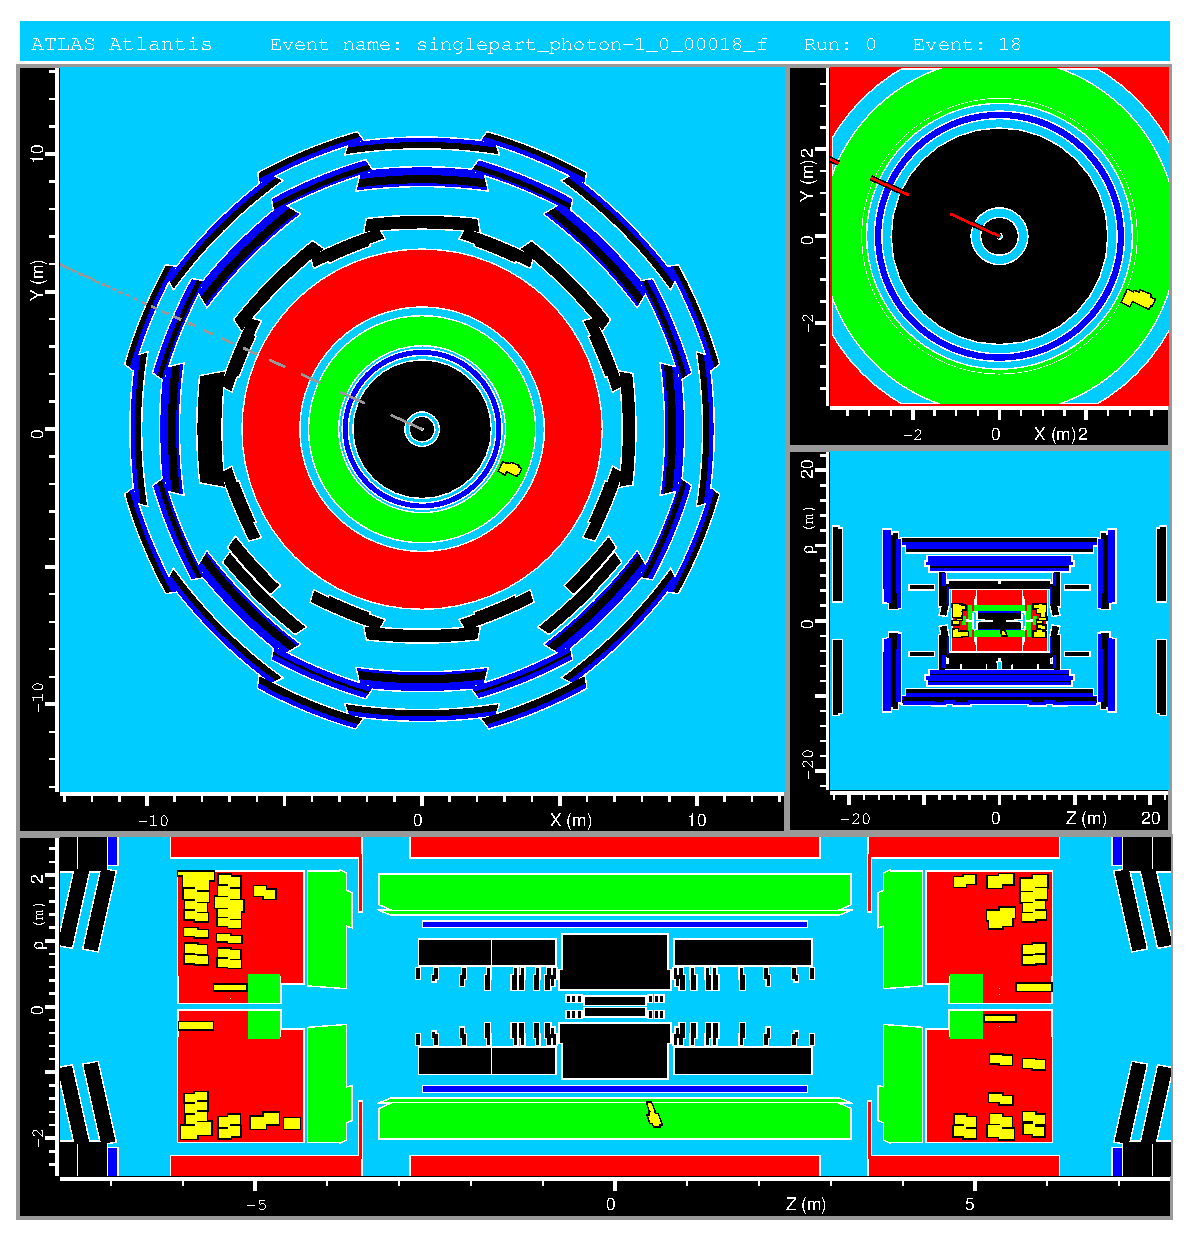
\includegraphics[width=0.6\textwidth]{photon_event18.eps}
    \caption{Event name: \texttt{singlepart\_photon-1\_0\_00018\_f}, Event: 18. }
    \label{fig:single_photon}
\end{figure}

We do not observe any signatures in the inner detector, but observe a single shower in the ECAL. This indeed matches the signature 
of a photon as they are electrically neutral and thus transparent to the tracking detectors. The energy deposition in each 
layer is around $E_T \approx 10 \sim 20 \si[]{\giga\electronvolt}$, indicating that the photon is energetic enough to undergo 
pair production or Compton scattering. \par 

\section{Tau Dataset}

Fig. \ref{fig:single_tau} shows Event 10 and 33 of the single dataset of the tau lepton. 

\begin{figure*}[htb!]
	\centering
	\subfloat[Event name: \texttt{singlepart\_tau-1\_0\_00010\_f}, Event: 10.]{{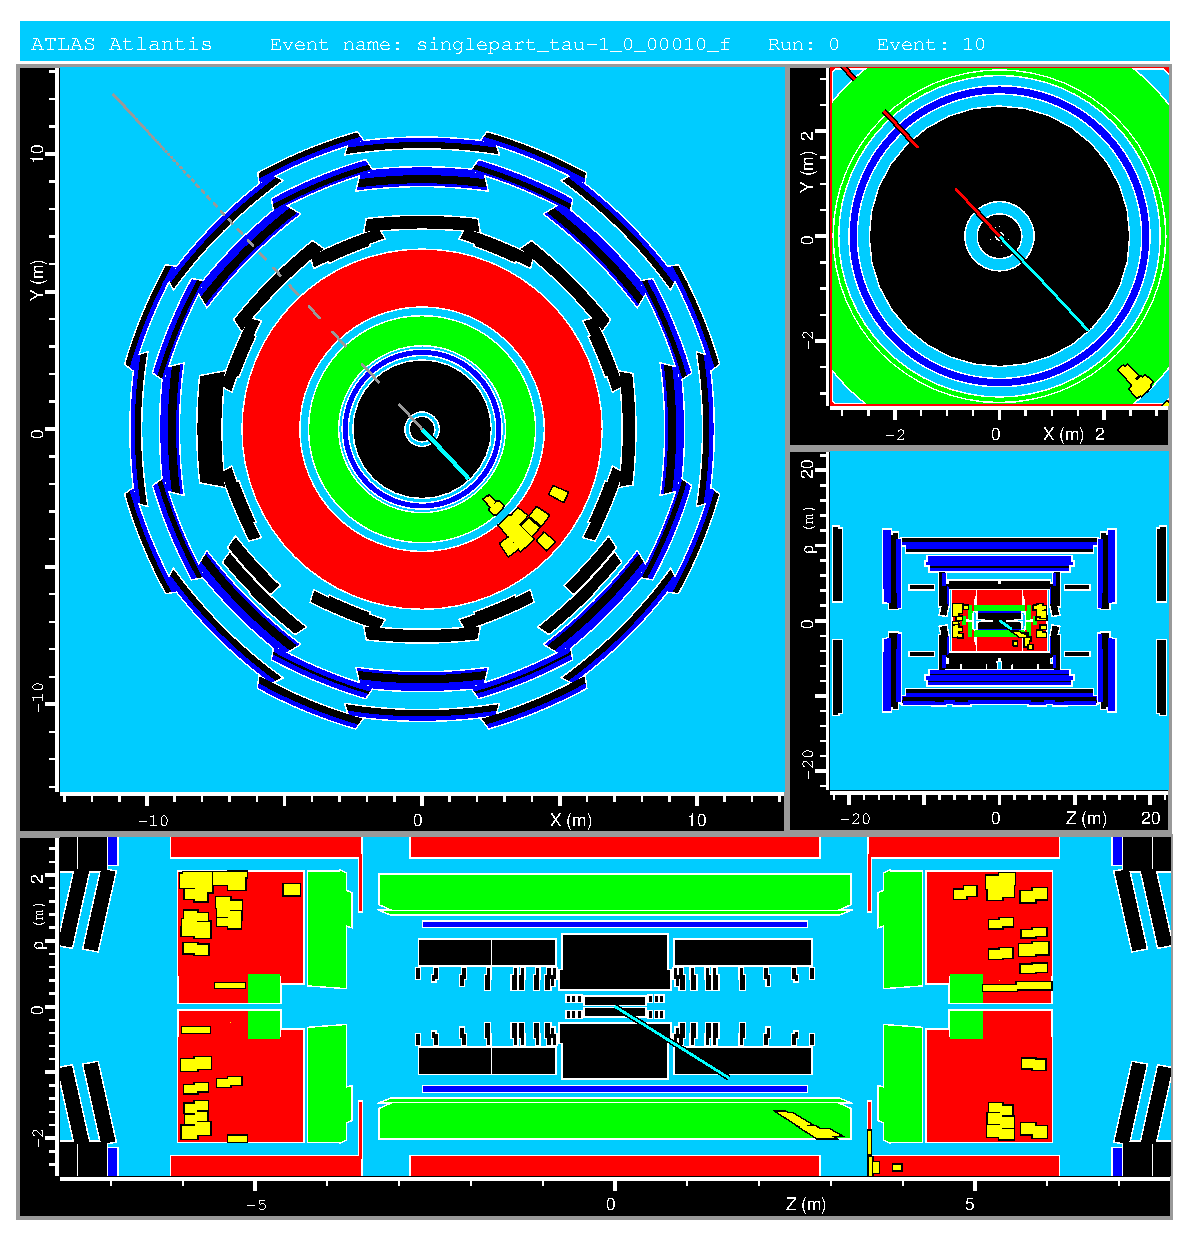
\includegraphics[width=0.47\columnwidth]{tau_event10.eps}}}
	\quad
	\centering
	\subfloat[Event name: \texttt{singlepart\_tau-1\_0\_00033\_f}, Event: 33.]{{\includegraphics[width=0.47\columnwidth]{tau_event33.eps}}}
	\caption{Signatures of tau leptons in the detector. (a) shows decays via hadrons and (b) shows signatures from leptonic decays.}
	\label{fig:single_tau}
\end{figure*}

In Event 10, we observe a collimated mini-jet that deposits signatures in both ECAL and HCAL. The energy deposition in the ECAL is 
most probably attributed to the photon pairs of the neutral pions produced within the mini-jets. The hadronic cascade in the HCAL is 
wide, which is due to the low momentum of the mini-jet ($ p_T = \SI{26.23 \pm 0.636}{\giga\electronvolt}$). The value of the missing 
$\slashed{E}_T$ is $\SI{ 28.298}{\giga\electronvolt}$, thus $\slashed{E}_T$ is most likely associated to the momentum of $\nu_\tau$. \par 

We further observe that in Event 33, we observe a leptonic decay process which is around 35\% of the branching ratio of 
the tau leptons. The event itself is indistinguishable from Event 7 in Fig. \ref{fig:single_muon}, thus making tau leptons that decay 
with this process much harder to detect. 

\section{Dijets Dataset}

We now observe events that display signatures of two jets in the detector. Fig. \ref{fig:dijets} shows Event 15 in the relevant dataset. 
The upper right lower plot shows the 2-D histogram between the pseudorapidity $\eta$ and azimuthal angle $\phi$ instead as it is more 
relevant for our discussion.

\begin{figure}[htpb]
    \centering
    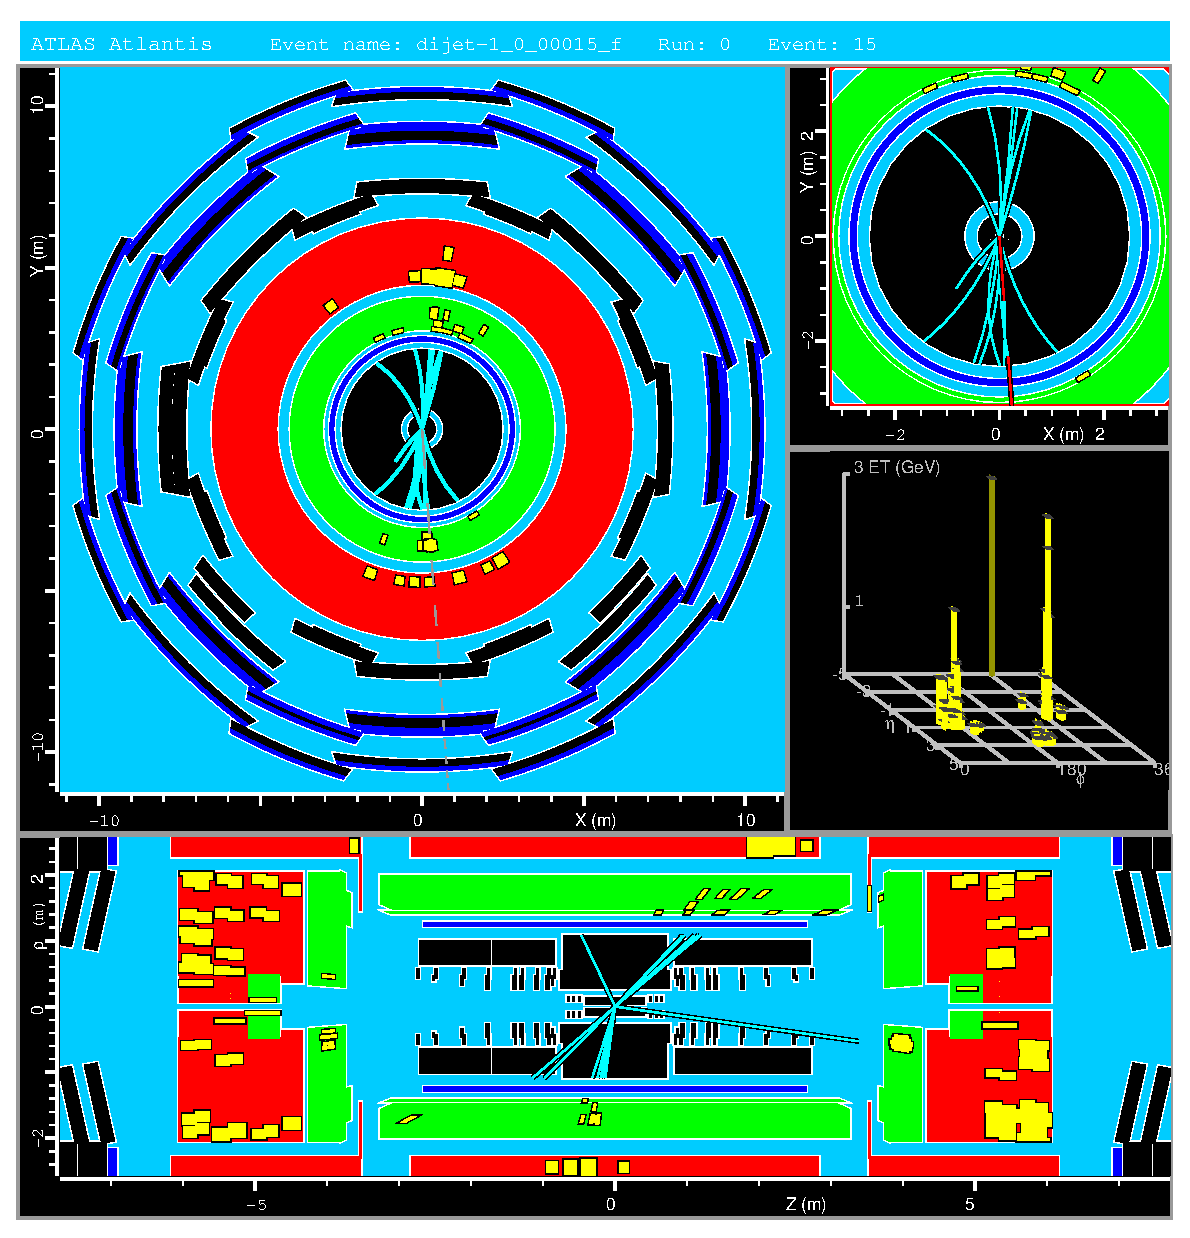
\includegraphics[width=0.6\textwidth]{dijet_event15.eps}
    \caption{Event name: \texttt{dijet-1\_0\_00015\_f}, Event: 15. }
    \label{fig:dijets}
\end{figure}

We observe two prominent jets generated opposite from each other in the transverse plane, where they are almost aligned with the y-axis.
 The two large peaks that are observed in the 2-D histogram also shows this behavior, where the azimuthal angle are approximately $180^\circ$ from each other. We can 
identify them as jets as they produce hadronic cascades at the HCAL. They also show signature in the ECAL which is mostly from semi-leptonic decays coming from $\tau$ lepton or b-jets and the photon
pairs due to neutral pion decays. We also observe two opposing trajectories (with opposing curvature) that only leave signatures
 in the ECAL. This is most probably an $e^+e^-$ pair that is generated by pair production of photons. When observing the lower plot, 
 we also observe an additional trajectory pair left to the lower jet with an energy deposition only in the ECAL.
  Using the ``pick'' command, we observe that the pairs have opposing curvatures with similar momenta, implying that these trajectories
  are from another $e^+e^-$ pair. 


\section{Wenu Data set}

In this data set, a $W$ boson decays like, $W^+ \rightarrow e^- \bar{\nu}_e$ or $W^+ \rightarrow e^+ \nu_e$. This means that the event will contain missing transverse momentum. In Fig. \ref{fig:wenu}, we see the event 9 from the data set. Starting from the vertex, we see two curved tracks in the top left figure, which deposit their energy in the ECAL. On the opposite side we also notice a huge deposition of hadrons in the HCAL. In the same direction, there is also the line for the $\vec{\slashed{E}_T}$. In the bottom figure, we see a huge number of deposits in the HCAL. 

\begin{figure}[htpb]
    \centering
    \includegraphics[width=0.6\textwidth]{Wenu-1_0_00009_f-YX-RZ-RZ-YX-2022-05-23-13-13-30}
    \caption{Event name: \texttt{Wenu-1\_0\_00009\_f}, Event: 9.}
    \label{fig:wenu}
\end{figure}

Since the event contains the decay $W \rightarrow e \nu$, one of the tracks which is opposite the $\vec{\slashed{E}_T}$ vector is mostly likely the electron from this decay. By using the pick function, we can see the details of $\vec{\slashed{E}_T}$, which are:

\begin{lstlisting}

ETMis:
 storegate key: MET_Final
 Sum-ET  = 45.688 GeV
 ET-Mis  = 31.907 GeV
 ETx-Mis = 25.086 GeV
 ETy-Mis = 19.716 GeV
 $\phi$ = 38.165$^{\circ}$
\end{lstlisting}
% The branching ratio (BR) of $W$ boson decay to jets is 67.46\% \cite{CMS:2022mhs}. Because of that we see a huge number of deposits in the HCAL for this event. For comparison, the BR of $W \rightarrow e \nu$ decay is 10.83\%. 

\section{WFull Data set}

Next, we study the \texttt{WFull-1-f.zip} data set. In this, all possible decays of $W$ boson can be seen. In Fig. \ref{fig:wfull}, starting from the vertex, several curved tracks emerge, indicating the presence of charged leptons and hadrons. Some curves disappear before reaching the ECAL, most likely due to their low momentum (sometimes called ``soft'' particles). The charged leptons leave their deposit in the ECAL and hadrons in the HCAL. For several deposits, we see an alignment, i.e., the jets contain leptons as well. This could be due to top quark, which decays to $t \rightarrow W^+ b$, from which we get jets from the $b$ quark and lepton and neutrino from the $W$. 

\begin{figure}[htpb]
    \centering
    \includegraphics[width=0.6\textwidth]{WFull-1_0_00005_f-YX-RZ-RZ-YX-2022-05-23-13-21-03}
    \caption{Event name: \texttt{WFull-1\_0\_00005\_f}, Event: 5.}
    \label{fig:wfull}
\end{figure}

The $\vec{\slashed{E}_T}$ is found to be 

\begin{lstlisting}

ETMis:
 storegate key: MET_Final
 Sum-ET  = 250.750 GeV
 ET-Mis  = 14.408 GeV
 ETx-Mis = -12.976 GeV
 ETy-Mis = 6.263 GeV
 $\phi$ = 154.236$^{\circ}$
\end{lstlisting}
which is quite high as compared to previous data set, indicating a high number of neutrinos and $W$ boson decays in the event. Further, there is a high number of deposits in the forward sections in the HCAL. This is an expected behavior, since the angular distribution of final state hadrons increases strongly in the forward region \cite{labman}. 

\section{Zee Data set}

Now we look at the \texttt{Zee-1-f.zip} data set. In Fig. \ref{fig:zee}, we see the event 3. Similar to our previous discussion, we see several tracks followed by deposits in ECAL and HCAL, with the presence of $\vec{\slashed{E}_T}$. An interesting feature of this data set is that several ECAL deposits are often opposite to each other. This means that the mother $Z^0$ boson was most likely at rest when these electrons were produced, giving us this characteristic. Using the pick function, we see that the transverse momentum of particles leaving a deposit in the ECAL opposite to each other are $31.23 \pm 1.028$ GeV and $-37.03 \pm 1.449$ GeV with an azimuthal angle of $\approx 174^{\circ}$ between them. 

\begin{figure}[htpb]
    \centering
    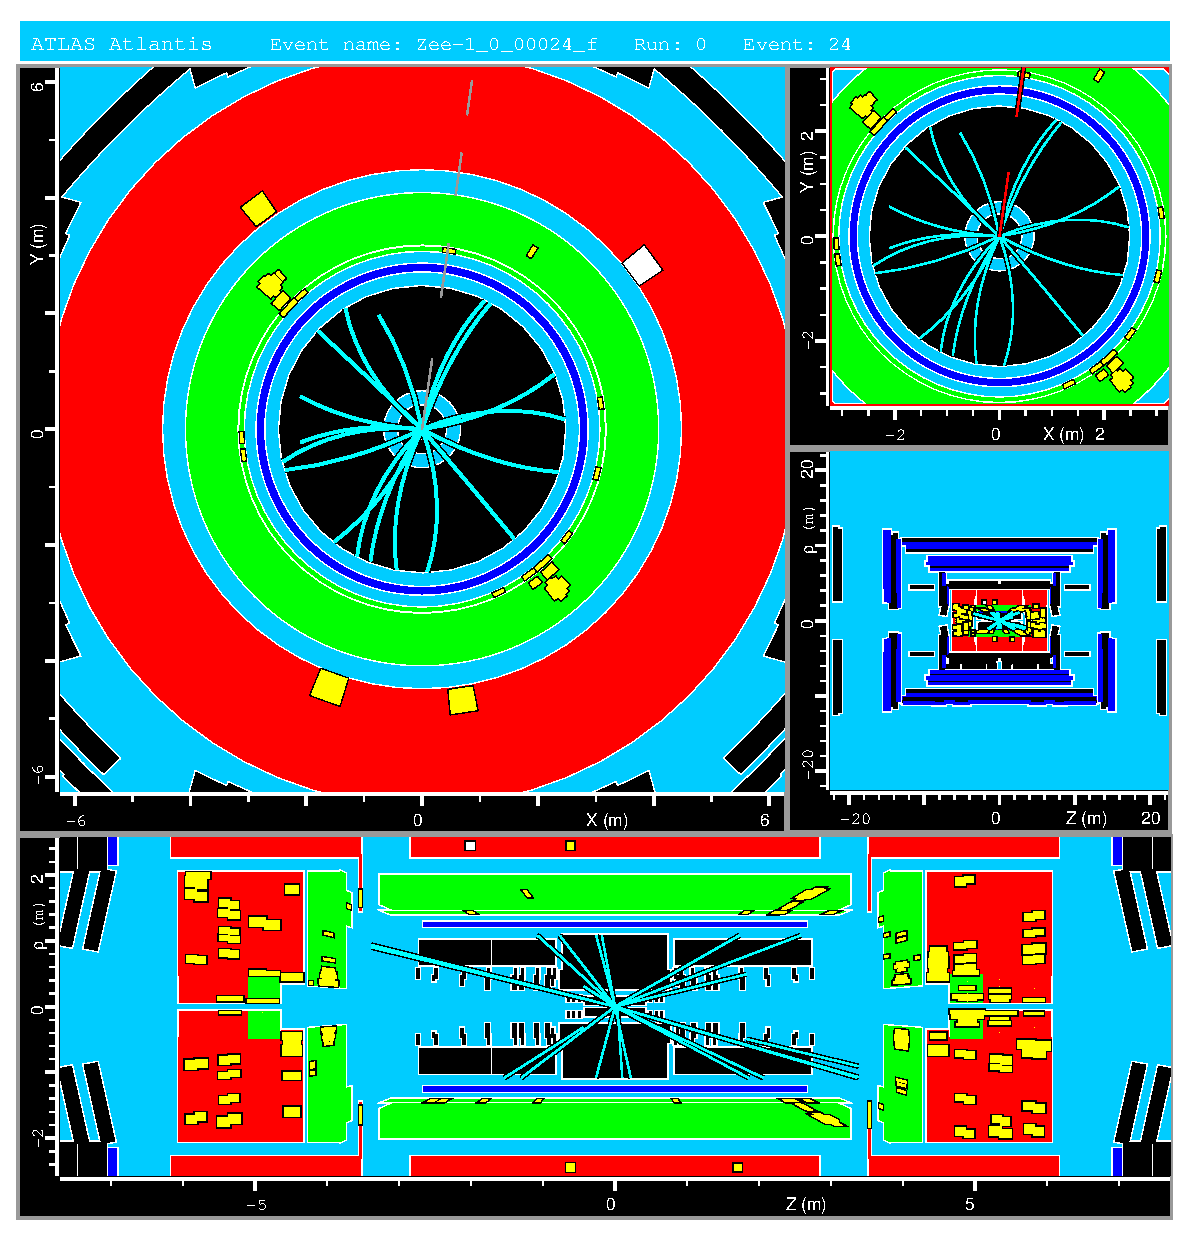
\includegraphics[width=0.6\textwidth]{Zee-1_0_00024_f-YX-RZ-RZ-YX-2022-06-28-02-09-55}
    \caption{Event name: \texttt{Zee-1\_0\_00003\_f}, Event: 24.}
    \label{fig:zee}
\end{figure}


Next, we work with two of the assignments listed in the lab manual. Since we were allowed to pick the assignments on our own, we chose to work with the \texttt{mystery-035-f.zip} data set and \texttt{ATLASData-Cosmics-M5.zip} data set. 

\section{Assignment 7: Mystery Data Set}  \label{subsec:mystery}
In this data set, a pre-selection is applied, in which at least two leptons ($e$ or $\mu$) are required to be in each event. The goal of this exercise is to look at the graphics and identify various Standard-Model processes by studying them. Further, we must try to rule out certain processes, if any. In Fig. \ref{fig:mys1}, we see the graphical view of event 13. Fig. \ref{fig:mys1_2}, gives us the zoomed in view of the vertex for the same event. We start our discussion from the vertex. 

A zoomed in view of the vertex shows that most tracks originate from the vertex, but some a reasonably far away from the vertex. The tracks originating far away from the vertex must come from a particle which has decayed after a certain period of time. This gives us the following three possibilities for the original particle: $\tau^{\pm}$ lepton, top quark or b-quarks (b-jet). Since $W$ and $Z^0$ boson decay almost immediately, the track reconstruction resolution would not be able to pick on the slight differences in the vertex due to those decays. 

As these particles start heading towards the detector, we see that charged particles are bent based on their momentum and leave a ``hit'' in the inner detector. Some particles are too ``soft'' and hence their tracks disappear before reaching the ECAL. Looking at the deposition at the ECAL and HCAL, we see that most depositions between them align with each other. This indicates the presence of charged electrons and photons in jets. We know that b-jets contain leptons, as in 25\% of all B decays, a lepton is produced. We can get this b-quark from the top quarks via $t \rightarrow W^+ b$. The figure in the bottom half also shows the presence of isolated jets, without leptons. Since $\tau$ leptons can decay purely to hadrons and neutrinos, one of the ways to identify them is to look for collimated ``mini'' jets. 
 
Two other interesting tracks we see in the ECAL and HCAL are the isolated depositions in ECAL which do not have a corresponding deposition in the HCAL. This means that these charged electrons can come from the following sources: photons, $W$ bosons, $Z^0$ bosons and $\tau$ leptons. The presence of missing energy in the event confirms the existence of neutrinos and hence, confirms the possibility of $W$ boson decays. The other interesting track corresponds to the deposition in HCAL and then a track in the muon detector. This confirms the presence of muons in the event, which was probably surrounded by jets. Ths could be either due to top quarks or b-quarks. 

\begin{figure}[htpb]
    \centering
    \includegraphics[width=0.6\textwidth]{mystery-035_0_00013_f-YX-RZ-RZ-YX-2022-05-23-13-28-39}
    \caption{Event name: \texttt{mystery-035-f}, Event: 13.}
    \label{fig:mys1}
\end{figure}

\begin{figure}[htpb]
    \centering
    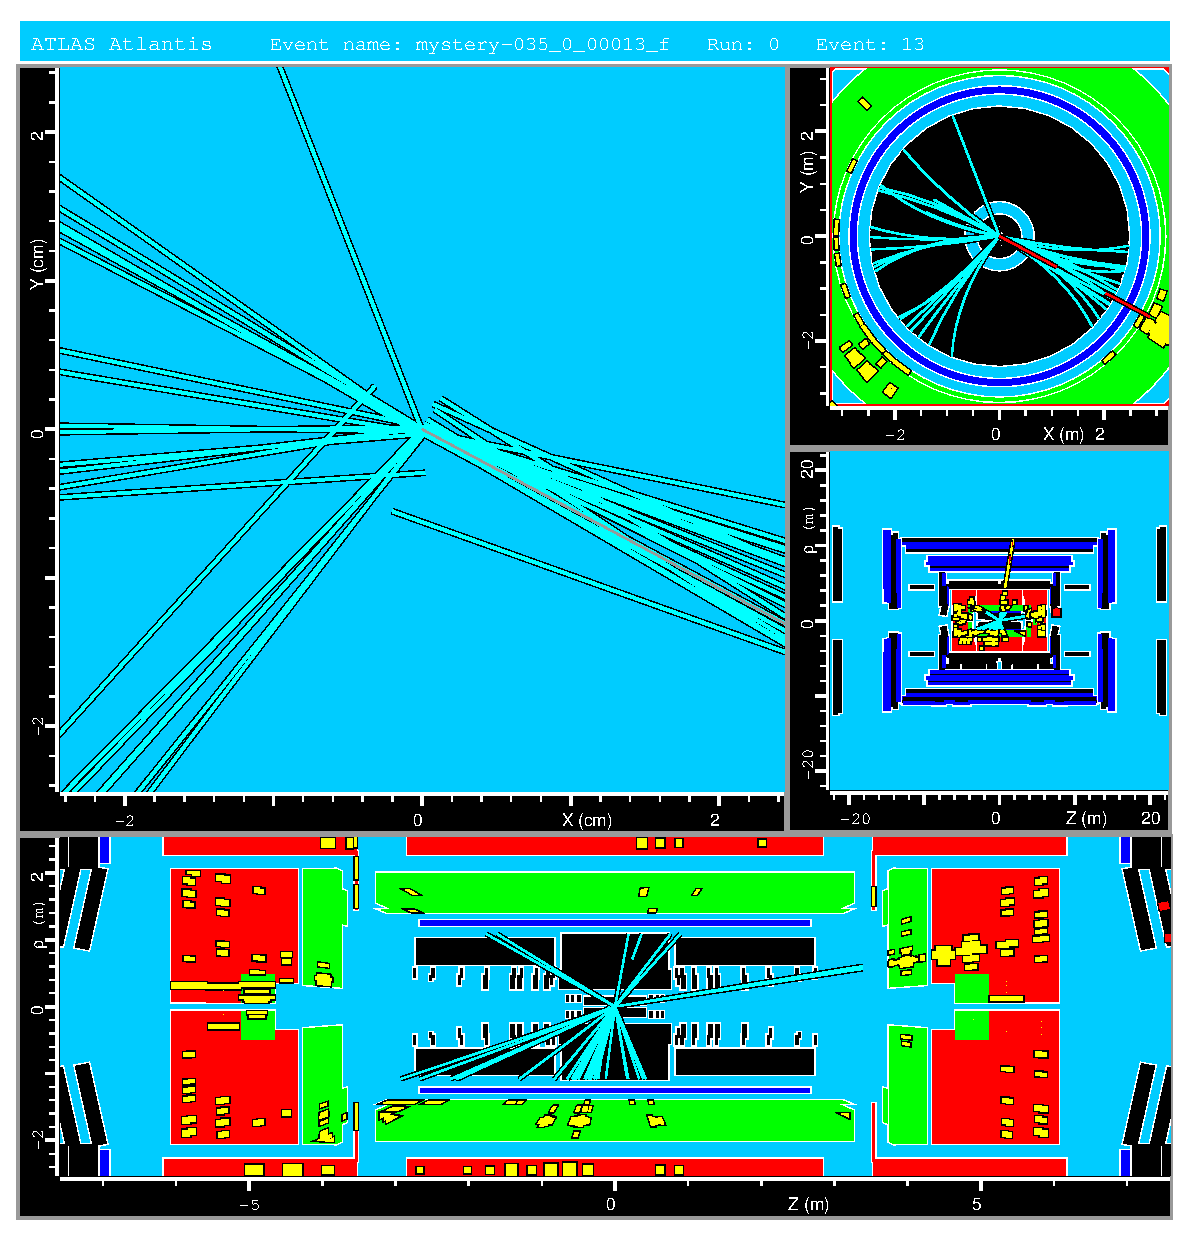
\includegraphics[width=0.6\textwidth]{mystery-035_0_00013_f-YX-RZ-RZ-YX-2022-05-23-13-34-34}
    \caption{Event name: \texttt{mystery-035-f}, Event: 13.}
    \label{fig:mys1_2}
\end{figure}


We look at one more event in Fig. \ref{fig:mys3}, event 12. In this event as well, we see all of the properties discussed above. Some thing which are slightly different is a higher number of isolated deposits in ECAL (without the corresponding deposit in HCAL) and the presence of two muons instead of a single one, both in the presence of jets. By selecting the missing energy track, we can look at the numbers. The following output was shown in the terminal: 

\begin{lstlisting}
ETMis:
 storegate key: MET_Final
 Sum-ET  = 1087.585 GeV
 ET-Mis  = 30.292 GeV
 ETx-Mis = -30.055 GeV
 ETy-Mis = 3.781 GeV
 $\phi$ = 172.829$^{\circ}$
 \end{lstlisting}

Since the $\slashed{E}_T$ is quite high, we can confirm the existence of one or more neutrinos in the event. Based on the discussion above, it is not possible to rule out any SM process for two lepton events. 


\begin{figure}[htpb]
    \centering
    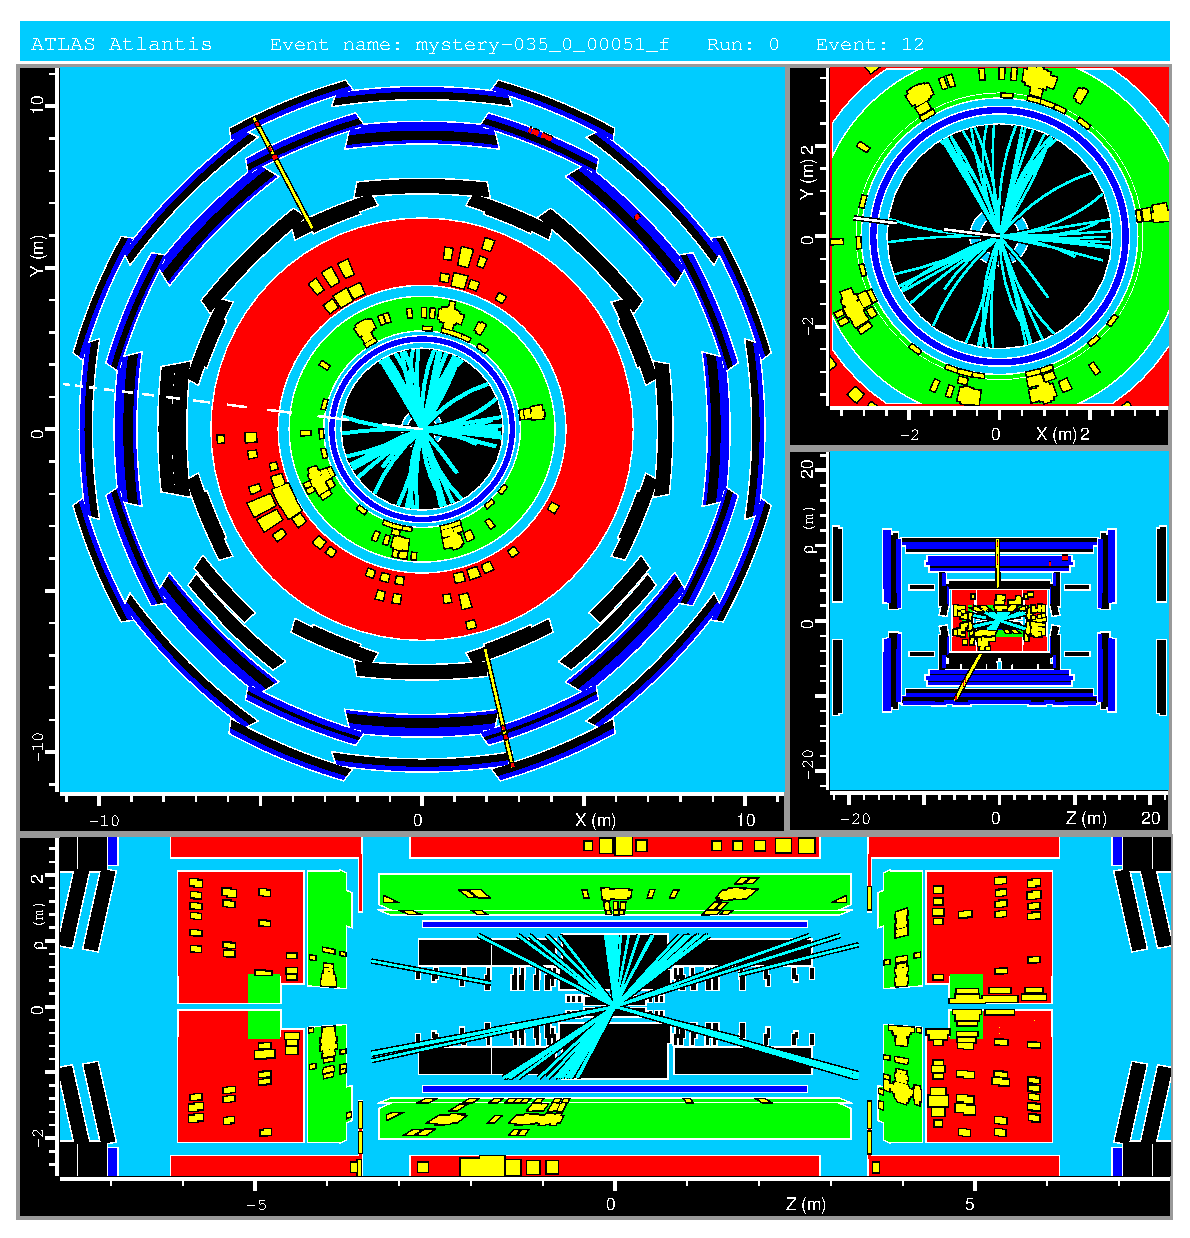
\includegraphics[width=0.6\textwidth]{mystery-035_0_00051_f-YX-RZ-RZ-YX-2022-06-18-17-20-41}
    \caption{Event name: \texttt{mystery-035-f}, Event: 12.}
    \label{fig:mys3}
\end{figure}

\section{Assignment 8: Cosmic Ray Dataset}

In this part of the assignment, we investigated the angular distribution 
of muons originating from pion decay from air showers in the atmosphere
that are detected from the muon chambers in the ATLAS detector. Real ATLAS data from 2007 and 
2008 was used in this assignment, contained in the provided file 
\texttt{ATLASData-Cosmics-M5.zip}. \par 

Fig. shows an example of an event observed with this dataset. Note that we have chosen different projections as compared to the figures 
shown in Sec. \ref{subsec:mystery} as the projections in such previous figures do not provide any new information in this assignment.
 We observe that no signatures have been observed in the inner detector as well as in both ECAL and HCAL. This is expected as these muons 
 have momentum of the order of 1 GeV, and as such they do not emit bremsstrahlung and thus no showers are formed in the calorimeters. \par 

\begin{figure}[htpb]
    \centering
    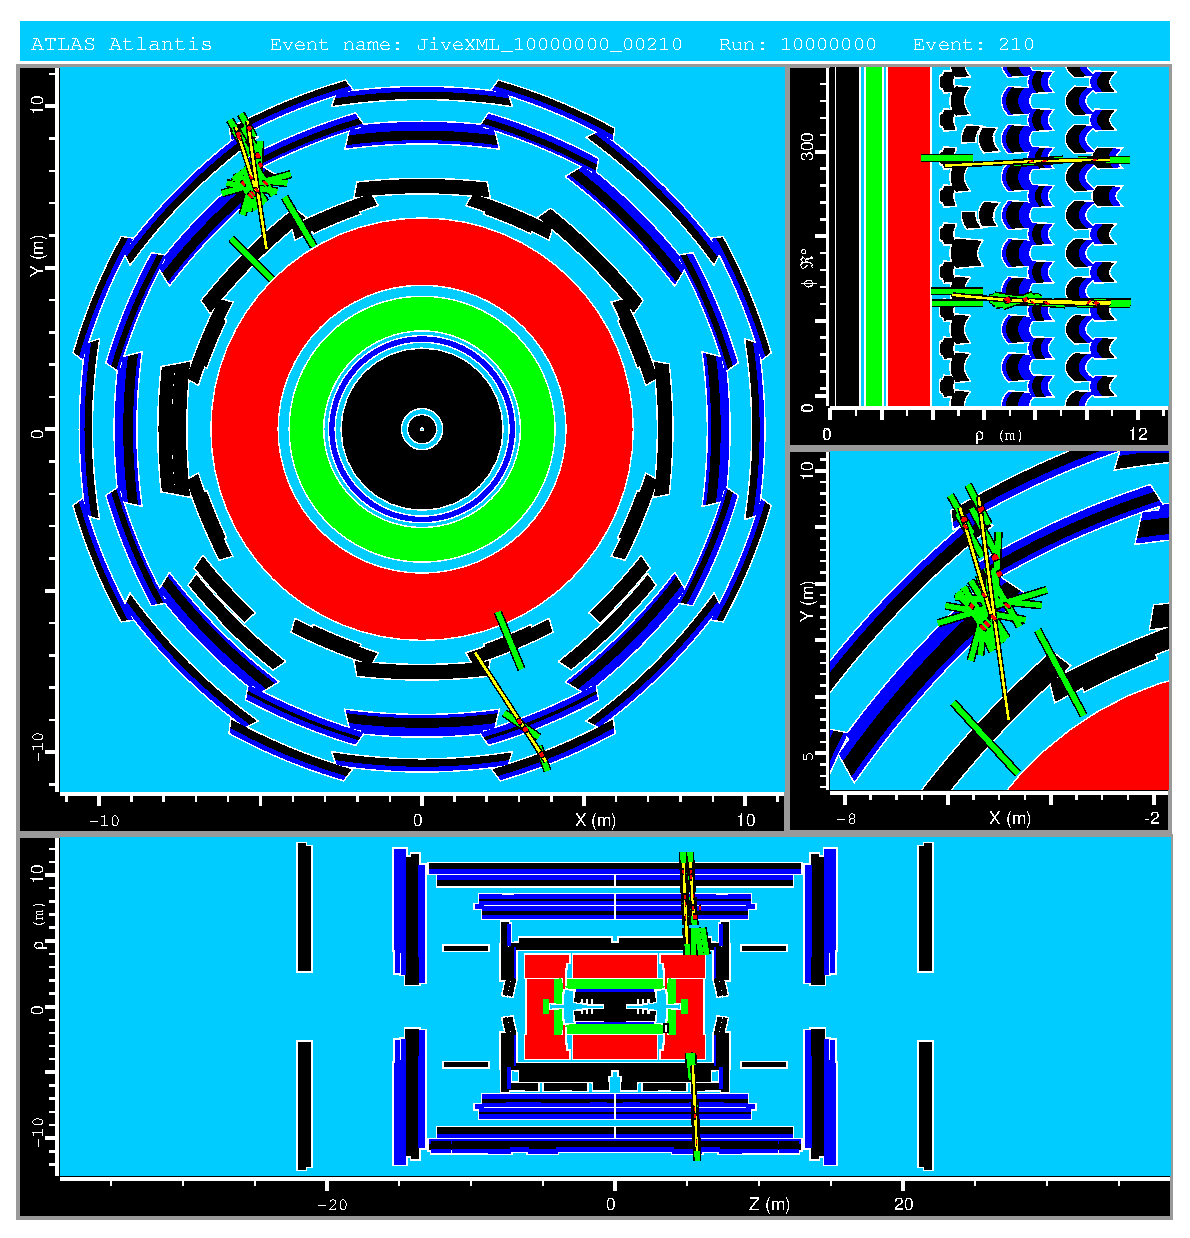
\includegraphics[width=0.55\textwidth]{muon_event210.eps}
    \caption{An example event for cosmic ray muons (Event 210). The reconstructed muon tracks are shown in yellow.}
    \label{fig:crevent210}
\end{figure}

To determine the angle in which the muon has entered the detector, we determined the azimuthal angle $\phi_0$ relative to the ATLAS detector. 
This is obtained by using the ''pick'' option in the \texttt{ATLANTIS} program to select each muon track in each event in this dataset. The azimuthal 
angle was then converted into the zenith angle, i.e. the angle from the local zenith. As $\phi_0 \in [0, 2\pi]$ where $\phi_0=0$ 
is at the positive x-axis, and $\theta \in [-\pi, \pi]$ where $\theta = 0$ is at the local zenith, an azimuthal angle of $\phi_0 = \pi / 2.$
will be equivalent to $\theta = 0$ as the local zenith is parallel to the y-axis in the detector. Following this logic, we can derive
the transformation between $\phi_0$ and $\theta$ as such: 
\begin{equation}
	\theta = 
	\begin{cases}
		\phi_0 - \frac{\pi}{2}   & : \phi_0 < \frac{3\pi}{2}\\
		(\phi_0 - \frac{\pi}{2}) - 2\pi & : \phi_0 > \frac{3\pi}{2}.
	\end{cases}
\end{equation}
See Appendix \ref{chap:appendix_figs} for a more detailed schematic of the transformation. \par 

Fig. \ref{fig:muon_angdist} shows the corresponding angular distribution from the cosmic ray muons observed in this dataset, along with the expected 
distribution $\cos^2 (\theta)$ at sea level. Note that we only plot from -90$^\circ$ to 90$^\circ$ as muons produced from beyond the horizon 
originate from air showers with an extremely low probability.\par 
\begin{figure}[htpb]
    \centering
    \includegraphics[width=0.7\textwidth]{muon_angdist.pdf}
    \caption{Angular distribution of cosmic ray muons observed from the ATLAS detector in 2007 and 2008. The expected $\cos^2 (\theta)$
	is also shown.}
    \label{fig:muon_angdist}
\end{figure}

We observe that while the muon intensity decrease with larger zenith angle, 
the distribution does not follow a $\cos^2 (\theta)$ distribution. This can be attributed to several reasons. Firstly, the ATLAS detector 
is located 100m below ground, and as such the muons with higher incoming angle will be stopped more by the underground material 
as compared to those near the zenith. Further, as there are two access shafts located above the ATLAS detector, muons with higher 
incoming angles interact less with underground material  \cite{Aad2011}. As such the distribution behaves like $\cos^n (\theta)$ with 
the exponent $n > 2$. Another reason for this is due to the low statistics, as the the total number of events is $N_{\mathrm{ev}} = 65$. 
With more events, the histogram will be smoother and thus will be able to discern whether the distribution behaves as $\cos^2(\theta)$
or not.\par 


\chapter{Calibration of Electrons} \label{chap:elec_calib}

Before performing the measurement of the $W$ mass, the data needs to be calibrated. In this experiment, the raw data was supplied to us and we first have to improve its quality. The most accurate way to determine the energy of electrons is by measuring the deposit in the ECAL. There are several reasons for calibration:

\begin{enumerate}
	\item The detector consists of hundreds of modules, which will return unequal energy. 
	\item There could be several parts of the calorimeter which might be inactive. 
	\item The electron loses a part of its energy in the silicon tracking region before depositing its energy in the calorimeter. 
\end{enumerate}
For these reasons, the raw energy values are lower than the true value. As such, we apply a calibration to fix these issues.

The mass of the $Z^0$ boson is a well known parameter of the SM. It has been measured to a precision of $2 \times 10^{-6}$ relative uncertainty. The width has been measured up to 1 per thousand. Further, we know that most of the electron-positron pairs in an event originate from $Z^0$. Hence, the $Z^0$ peak, which is a well known signal, can be used in order to calibrate our data. 

To perform this calibration, we use the library \texttt{fitZee.C}, which takes the calibration from the file \texttt{ElecCalib.C} and applies that to the data. Applying changes to the \texttt{ElecCalib.C} file and compiling \texttt{fitZee.C} also changes the \texttt{z.Fit()} command. After activating \texttt{root}, the following commands are run:

\begin{verbatim}
.L fitZee.C+
fitZee z
z.Fit("")
\end{verbatim}
This creates a calibration object \texttt{z} which will be used to calibration. The \texttt{z.Fit("")} command fills the histogram and applies the best fit and outputs the fit parameters. The output of this command is shown in Fig. \ref{fig:uncalib}. The $Z^0$ mass for the uncalibrated data is found to be $89.87 \pm 0.02$ GeV and resolution is $2.588 \pm 0.026$. In the calibration process, the aim is to get the mass as close as possible to the ideal value, which is $91.1876 \pm 0.0021 \ \text{GeV}$. Further, the resolution should also be decreased by at least 0.2, while trying to get a good $\chi^2 / ndf$ value ($ndf$ stands for number of degrees of freedom). A value of approximately 1 is ideal. $\chi^2$ characterizes the fit quality and the aim is to usually minimize it. Therefore, a high $\chi^2$ signifies a bad fit. 

\begin{figure}[htpb]
    \centering
    \includegraphics[width=0.8\textwidth]{uncalib}
    \caption{The output of the uncalibrated data. A resonance near the $Z^0$ mass can be seen. The red line is the fit and the legend contains the fit parameters.}
    \label{fig:uncalib}
\end{figure}

One can also look at fits with cuts, i.e., looking at how the fit changes for different regions of the parameter spectrum. For instance, to look at the fit in the different regions of the azimutal angle $\phi$, the following command can be run

\begin{verbatim}
z.Fit("el_phi>0. && el_phi<0.4")
\end{verbatim}
Thus, passing the cuts in the fit command allows us to probe different regions of the parameters. Some of the available variables are \texttt{el\_pt} (transverse momentum of electron), \texttt{el\_eta} (psuedorapidity), \texttt{el\_energy} and several others. After applying cuts in several ranges, one can run \texttt{z.List()} and looking at the numbers corresponding to different ranges, stack them in the single plot by running

\begin{verbatim}
z.Draw(0, 1, 2, 3)
\end{verbatim}

\begin{figure*}[htb!]
	\centering
	\subfloat[Stacked reconstructed fits of different azimuthal angle, $\phi$, regions. \label{subfig:phi-range}]{{\includegraphics[width=0.47\columnwidth]{phi-range}}}
	\quad
	\centering
	\subfloat[Stacked reconstructed fits of different pseudorapidity, $|\eta|$, regions in {[}0, 2.5{]} in 0.5 increments. \label{subfig:eta-range}]{{\includegraphics[width=0.47\columnwidth]{eta-range}}}
	\caption{Stacked plots of different parameters in different regions. We notice a shift in the peak for different regions.}
	\label{fig:region-stack}
\end{figure*}

An example of this is shown in Fig. \ref{fig:region-stack}. A shift in the peak can be seen for different regions. These regions must be studied and calibration must be applied to them. After applying the calibration for several regions, the output is observed and the process is repeated for several more regions and variables. After several trail and errors, we were able to get the desired calibration. 

After applying cuts for different regions of a single variable, the calibration was applied and the output was looked at. Then, with this applied calibration, different regions of another variable were compared as mentioned above and the calibration file was modified to correct for this variables. This was done for these set of variables in the following order: \texttt{phi, eta, mindrjet} (which is the minimum distance of the electron to the nearest jet in the $\eta \phi$ plane), \texttt{etiso} (transverse energy of the electron in the area surrounding it in the calorimeter) and \texttt{pt} (transverse momentum). The corresponding plots are shown in Fig. \ref{fig:calib-process} and the final calibration plot is shown in Fig. \ref{fig:final-calib}. The corresponding code can be found in the Appendix \ref{chap:appendix_code}. 
\begin{figure*}[htb!]
	\centering
	\subfloat[Calibration for only different regions of $\phi$. \label{subfig:phi-calib}]{{\includegraphics[width=0.47\columnwidth]{phi_calib}}}
	\quad
	\centering
	\subfloat[Calibration for $\phi$ followed by $|\eta|$. \label{subfig:eta-calib}]{{\includegraphics[width=0.47\columnwidth]{phi_eta_calib}}}
	\quad
	\centering
	\subfloat[Calibration for $\phi$ and $|\eta|$ followed by \texttt{mindrjet}. \label{subfig:rjet-calib}]{{\includegraphics[width=0.47\columnwidth]{phi_eta_rjet}}}
	\quad
	\centering
	\subfloat[Calibration for $\phi$, $|\eta|$, \texttt{mindrjet} followed by \texttt{etiso}. \label{subfig:etiso-calib}]{{\includegraphics[width=0.47\columnwidth]{phi_eta_rjet_etiso}}}
	\caption{Calibration applied one after the other for different set of variables.}
	\label{fig:calib-process}
\end{figure*}

\begin{figure}[htpb]
    \centering
    \includegraphics[width=0.8\textwidth]{final_calib_fit}
    \caption{The final fit curve after applying $\phi$, $|\eta|$, \texttt{mindrjet}, \texttt{etiso} followed by $p_T$ calibrations.}
    \label{fig:final-calib}
\end{figure}

Thus, we were able to get the mass to be $91.198 \pm 0.0196$ GeV and the resolution to be $2.342 \pm 0.024$. $\chi^2/ndf$ is found to be $464.6 / 172 \approx 2.7$. Using the command \texttt{z.Compare()}, we can see the effect of calibration on the data, in Fig. \ref{fig:calib-compare}. Further, we also notice a change in the values of mass, resolution and $\chi^2/ndf$. This is because the \texttt{Compare()} function uses the ``LARGE'' argument in the Fit() function, which uses all the data. By running \texttt{z.Fit("","LARGE")}, the change in the values was confirmed. 

\begin{figure}[htpb]
    \centering
    \includegraphics[width=0.8\textwidth]{calib_compare}
    \caption{Comparison between calibrated and uncalibrated data. The blue fit corresponds to calibrated data and the green to the uncalibrated data.}
    \label{fig:calib-compare}
\end{figure}

\chapter{Measurement of the $W$ boson Mass} \label{chap:wboson}

In this section, we elaborate on the methods used to determine the $W$ boson mass using real ATLAS data. As mentioned in Sec. 
\ref{sec:gauge_bosons}, there are several methods to determine the mass of the $W$ boson. In this experiment, we measure this 
mass by observing the position of the Jacobi peak from the electron $p_T$ distribution resulting from $W \rightarrow e\nu$ 
events. \par 

In this experiment, we were given several datasets, mostly containing simulated $W \rightarrow e\nu$ events with 
different $W$ boson masses and real ATLAS data for the same process. A dataset containing real ATLAS data 
from $Z \rightarrow ee$ events are also contained, used to verify that the gauge curves retrieve the $Z^0$ boson mass accurately, which 
is known more accurately than the $W$ boson mass. A list of the datasets is shown in Table \ref{tab:datasets}. 

\begin{table}
    \centering
    \begin{tabular}{|c|c|}  \hline
     Dataset Abbrv.& Description    \\ \hline
     \texttt{Wenu} &  Real ATLAS data for  $W \rightarrow e\nu$ candidate events \\
     \texttt{Zee} &  Real ATLAS data for  $Z \rightarrow ee$ candidate events  \\ 
     \texttt{MCW75} &  Simulated events with $m_W = \SI{75}{\giga\electronvolt}$ \\ 
     \texttt{MCW78} &  Simulated events with $m_W = \SI{78}{\giga\electronvolt}$ \\ 
     \texttt{MCW79} &  Simulated events with $m_W = \SI{79}{\giga\electronvolt}$ \\ 
     \texttt{MCW / MCW80} &  Simulated events with $m_W = \SI{80}{\giga\electronvolt}$ \\ 
     \texttt{MCW81} &  Simulated events with $m_W = \SI{81}{\giga\electronvolt}$ \\ 
     \texttt{MCW82} &  Simulated events with $m_W = \SI{82}{\giga\electronvolt}$ \\ 
     \texttt{MCW85} &  Simulated events with $m_W = \SI{85}{\giga\electronvolt}$ \\ 
     \texttt{QCD} & QCD background events extracted from ATLAS data \\ 
     \texttt{non-QCD} & non-QCD backgrounds obtained from simulated data \\ \hline
    \end{tabular}
    \caption{List of datasets available for this experiment. The abbreviation used to use such datasets in ROOT is 
    provided.}
    \label{tab:datasets}
\end{table}

In addition to the $W$ and $Z^0$ boson datasets, two additional datasets relating to the QCD and non-QCD backgrounds are contained. The QCD
background dataset are generated from proton-proton collisions where the hard interactions are strong. As it is difficult to 
simulate the QCD events containing electrons, this background is extracted directly from real ATLAS data instead. While this matches the 
shape of the QCD backgrounds in the $W$ and $Z^0$ boson datasets, the integrated luminosity are not equal and thus a proper normalization
using a scale factor is required for our analysis. The non-QCD backgrounds are extracted from simulated events \cite{labman}. \par 

For all parts of the analysis, we use ROOT and use the C++ library \texttt{Wenu.C+} to load the C++ object used in the analysis. 
This is loaded with the following commands:
\begin{verbatim}
    .L Wenu.C+ 
    Wenu w
\end{verbatim} 


\section{Verification of Electron Calibration}

We first verify our calibration of the electron momentum performed in Chap. \ref{chap:elec_calib}. This is done by 
running the \texttt{FitZee} function which acts similarly to the \texttt{z.Fit} function in Chap. \ref{chap:elec_calib}. We observed 
this distribution for 4 kinematical regions of interest. The obtained histogram from applying no cuts is shown in Fig. \ref{fig:zee_calib}. 

\begin{figure}[htpb]
    \centering
    \includegraphics[width=0.9\textwidth]{zeefit.pdf}
    \caption{The invariant mass distribution of $ee$ from $Z \rightarrow ee$ decays without applying any cuts. The blue points are the 
    real data from ATLAS, the red line is the curve fit, and the green histogram is the simulated data. The background 
    is also shown in yellow.}
    \label{fig:zee_calib}
\end{figure}

We observe that the invariant mass for the $e^+ e^-$ pair is given as $\SI{91.17 \pm 0.01}{\giga\electronvolt}$, which agrees with the 
world average value of the $Z^0$ boson mass of $\SI{91.1876 \pm 0.0023}{\giga\electronvolt}$ within $1.76\sigma$ \cite{ParticleDataGroup:2020ssz}.
One of the reason for this deviation may be due to the fact that the scaling for the calibration was only performed to two significant digits. The mass values themselves yield similar results and thus we agree that the calibration is properly applied. \par 

We also observe the invariant masses for the same distribution with different cuts: \texttt{el\_energy} $<$ 50 ($E_e < \SI{50}{\giga\electronvolt}$), \texttt{el\_eta} $<$ 1 
($\eta < 1$), and \texttt{el\_pt} $<$ 40 ($p_{T_e} < \SI{40}{\giga\electronvolt}$). See Appendix \ref{chap:appendix_figs} for the 
invariant mass distributions for each cut. From these distributions, we obtain the following invariant masses for each cut 
respectively: 
$\SI{90.93 \pm 0.02}{\giga\electronvolt}$, $\SI{91.14 \pm 0.01}{\giga\electronvolt}$, $\SI{90.94 \pm 0.02}{\giga\electronvolt}$. 
When comparing with the world average value, we observe that they are also close to the $Z^0$ boson mass, with the largest deviation 
of $\SI{0.25}{\giga\electronvolt}$. This shows that even with cuts applied, the $Z^0$ boson mass is calibrated to an acceptable range. 

\section{Kinematic Parameters and Preliminary QCD Scaling}

Once we have verified that our calibration is properly applied, we observe the distributions for ATLAS data compared with 
simulated data for different relevant parameters. In our analysis, we observed the following parameters: 
\texttt{el\_pt}, \texttt{el\_etiso}, \texttt{njet}, \texttt{etmis}, and \texttt{ptw}. In the following sections, we highlight
the importance of each parameter. The distributions were constructed by the following command:
\begin{verbatim}
    w.PlotW(PARAMETER, BINS, XMIN, XMAX, CUTS).
\end{verbatim} 
The transverse momentum distribution for electrons, which is most relevant to us for determining the Jacobi peak, is shown 
in Fig. \ref{fig:elpt_nocuts}. See Appendix \ref{chap:appendix_figs} for the distributions for the other parameters with no cuts applied. \par 

\begin{figure}[htpb]
    \centering
    \includegraphics[width=0.8\textwidth]{elpt_nocuts.pdf}
    \caption{The transverse momentum distribution for electrons for the $W$ boson decay with no cuts applied. The blue points are the ATLAS data, 
    the green histogram is the simulated $W \rightarrow e\nu$ decays, and the yellow and purple histograms are the QCD and 
    non-QCD backgrounds respectively.}
    \label{fig:elpt_nocuts}
\end{figure}

From the $p_T$ distribution of electrons, we observe that the amplitude of the simulated data (and the backgrounds) are much 
higher than the real data. This is caused by the uncalibrated scaling of the QCD background, and as such we set a scale factor 
so that the two data coincide. To do this, we use the function \texttt{w.SetQCDScaleFactor(VALUE)} and we set a preliminary 
value of 0.3. See Fig. \ref{fig:elpt_qcd30} for the effect on applying such scale factor to the electron $p_T$ distribution. In the following sections, we will refine the scaling parameter after applying cuts and setting fitting ranges. \par

\begin{figure}[htpb]
    \centering
    \includegraphics[width=0.8\textwidth]{elpt_qcd30.pdf}
    \caption{Same as Fig. \ref{fig:elpt_nocuts} but applying the QCD scale factor of 0.3 instead.}
    \label{fig:elpt_qcd30}
\end{figure}

 

To obtain a sharp Jacobi peak, we want to reduce the smearing of the peak as much as possible. One factor that contributes 
to such smearing is the transverse momentum of the $W$ boson $p_{T_W}$ as mentioned in Sec. \ref*{sec:gauge_bosons}. To reduce this, 
we filter events in which several jets are produced. The $W$ bosons obtained from such events suffer recoil from the quarks and gluons 
produced with the proton-proton collision, yielding a finite $W$ boson transverse momentum. This is shown in the $p_{T_W}$ distribution 
for different number of jets in Figs. \ref{fig:ptw_njet0} and \ref{fig:ptw_njets}. For events with no jets, the distribution is 
sharply peaked close to zero, however the peak shifts to $p_{T_W} \approx \SI{50}{\giga\electronvolt}$ for events with one or more jets. 
We also observe that the number of events decrease as we increase the number of jets, indicating that most events in this dataset are those without any jets. We further observe from these distributions that the QCD background increases as the number of jets increase due to the number of QCD processes involved. For the distributions with 
three and four jets, the QCD background overlaps the simulated data itself.  

\begin{figure}[htpb]
    \centering
    \includegraphics[width=0.8\textwidth]{ptw_qcd30_njet0.pdf}
    \caption{Transverse momentum distribution for $W$ boson in $W$ boson decay with no jets. The color code follows from Fig. \ref{fig:elpt_nocuts}.}
    \label{fig:ptw_njet0}
\end{figure}

\begin{figure*}[htb!]
	\centering
	\subfloat[\texttt{njet == 1}]{{\includegraphics[width=0.47\columnwidth]{ptw_qcd30_njet1.pdf}}}
	\quad
	\centering
	\subfloat[\texttt{njet == 2}]{{\includegraphics[width=0.47\columnwidth]{ptw_qcd30_njet2.pdf}}}
	\quad
    \centering
	\subfloat[\texttt{njet == 3}]{{\includegraphics[width=0.47\columnwidth]{ptw_qcd30_njet3.pdf}}}
	\quad
    \centering
	\subfloat[\texttt{njet == 4}]{{\includegraphics[width=0.47\columnwidth]{ptw_qcd30_njet4.pdf}}}
	\quad
	\caption{Same as Fig. \ref{fig:ptw_njet0} but for finite number of jets. }
	\label{fig:ptw_njets}
\end{figure*}

From such plots, we observe that in order to reduce $p_{T_W}$ and thus reduce the smearing of the Jacobi peak,
 we should set a cut of the number of jets such that events with no jets are chosen. 
 
\section{QCD Scale Factor and Cut Selection}   \label{sec:qcdscale_cuts}

In order to properly set the QCD scale factor, we use the \texttt{el\_etiso} distribution. The parameter \texttt{el\_etiso} 
represents the number of electrons observed within a cone of jets with $\Delta R = \sqrt{(\Delta \eta)^2 + (\Delta\phi)^2} < 0.45$. 
This parameter is relevant as it quantifies the amount of QCD background events surrounding the electrons used to construct the 
electron $p_T$ distribution. Thus to scale the QCD background, we observe the distribution where \texttt{el\_etiso} $< \SI{10}{\giga\electronvolt}$.
In our analysis, we set the scale factor to be 0.30. Fig. \ref{fig:etiso_qcd} shows the \texttt{el\_etiso} distribution in the full range 
and in the high QCD background range before and after setting the scale factor. We observe that applying our set scale factor 
yields amplitudes close to the real ATLAS data. \par 

\begin{figure*}[htb!]
	\centering
	\subfloat[Full range, before scaling]{{\includegraphics[width=0.47\columnwidth]{etiso_nocuts.pdf}}}
	\quad
	\centering
	\subfloat[High QCD background region, before scaling]{{\includegraphics[width=0.47\columnwidth]{etiso_nocuts_1020.pdf}}}
	\quad
    \centering
	\subfloat[Full range, after scaling]{{\includegraphics[width=0.47\columnwidth]{etiso_qcd30.pdf}}}
	\quad
    \centering
	\subfloat[High QCD background region, after scaling]{{\includegraphics[width=0.47\columnwidth]{etiso_qcd30_1020.pdf}}}
	\quad
	\caption{\texttt{el\_etiso} distribution before scaling (top) and after scaling (bottom) for the whole distribution (left)
    and in the region with high QCD background (right). The QCD scale factor was set to 0.30.}
	\label{fig:etiso_qcd}
\end{figure*}

To estimate the uncertainty due to the QCD scale factor, we varied the scale factor until the deviation between the real data 
and the simulated data was significant (by eye). From this we chose that the scale factor is acceptable between 0.28 and 
0.32. See Appendix \ref{chap:appendix_figs} for the distributions in the full range 
and in the high QCD background region for the two scale factors mentioned. This will be important in quantifying the systematic 
errors for the $W$ boson mass. \par 

From the above discussion, we require that we need to have events with no jets to reduce the transverse momentum of the $W$ boson and 
to have \texttt{el\_etiso} $< \SI{10}{\giga\electronvolt}$ to reduce events from the QCD background. After investigating the optimal 
value of \texttt{el\_etiso}, we set the following cuts: \texttt{njet == 0} and \texttt{el\_etiso $<$ 8}. Fig. \ref{fig:ptw_cuts} show 
the $p_{T_W}$ distribution before and applying such cuts. We also verified that after applying 
such cuts, the QCD scaling factor is still valid. From this figure we observe that the impact from the QCD backgrounds 
is suppressed in higher $p_{T_W}$ values as expected. 

\begin{figure*}[htb!]
	\centering
	\subfloat[No cuts]{{\includegraphics[width=0.47\columnwidth]{ptw_qcd30.pdf}}}
	\quad
	\centering
	\subfloat[After cuts, \texttt{njet == 0, el\_etiso $<$ 8}]{{\includegraphics[width=0.47\columnwidth]{ptw_qcd30_njet0_etiso8.pdf}}}
	\caption{$W$ boson transverse momentum distribution (a) before and (b) after applying cuts. The cuts \texttt{njet == 0, el\_etiso $<$ 8}
    was applied.}
	\label{fig:ptw_cuts}
\end{figure*}

\section{Gauge Curve}

We now apply the fit provided in ROOT to obtain the half-maximum of the electron $p_T$ distribution. This was performed using the 
command \texttt{w.GetHalfMaximum(DATASET, XMIN, XMAX)} for each simulated dataset given in Table \ref{tab:datasets}, 
corresponding to masses $m_W =$ 75, 78, 79, 80, 81, 82, and 85 $\si{\giga\electronvolt}$. To efficiently run this portion 
of the analysis, a macro file \texttt{WMacro.C} was constructed (see Appendix \ref{chap:appendix_code}). The resulting half-maximum plots 
for each mass is shown in Appendix \ref{chap:appendix_figs}. Here we show the results for $m_W = \SI{80}{\giga\electronvolt}$ as 
an example, shown in Fig \ref{fig:hm_m80}. For this analysis, we used the fitting range of [28, 60].

\begin{figure}[htb!]
    \centering
    \includegraphics[width=0.6\textwidth]{hm_80.pdf}
    \caption{Half-maximum fit of electron $p_T$ spectrum for simulated data with $m_W = \SI{80}{\giga\electronvolt}$.}
    \label{fig:hm_m80}
\end{figure}

Once we obtain the half-maximum from each fit, we apply a linear fit to directly relate the mass of the $W$ boson and the 
obtained half-maximum $h$ as such: 
\begin{equation}
    h = a \cdot m_W + b
    \label{eq:half_max}
\end{equation}

\begin{figure}[htpb!]
    \centering
    \includegraphics[width=0.7\textwidth]{gauge_curve.pdf}
    \caption{Gauge curve between half-maximum from fit with simulated data against $W$ boson mass.}
    \label{fig:gauge_curve}
\end{figure}

This line is called the gauge curve. The corresponding gauge curve for the seven masses is shown in Fig. \ref{fig:gauge_curve}. The 
linear fit was evaluated by the Python module \texttt{lmfit} that utilizes the Levenberg-Marquardt method. Table \ref{tab:gauge_params} 
shows the obtained parameters from the fitting procedure.

\begin{table}[htb!]
    \centering
    \begin{tabular}{|c|c|c|} \hline
    a & b [$\si{\giga\electronvolt}$] &  $\chi^2$  \\ \hline
    $0.5214 \pm 0.0080$ & $1.04 \pm 0.64$  & 8.68  \\ \hline
    \end{tabular}
    \caption{Parameters obtained from fitting the gauge curve.}
    \label{tab:gauge_params}
\end{table}

The covariance matrix obtained from the fit is shown as such: 
\begin{equation}
    \begin{pmatrix}
        \sigma_a^2 & \sigma_{ab} \\ 
        \sigma_{ab} & \sigma_b^2 
    \end{pmatrix}
    =
    \begin{pmatrix}
        \num{6.48e-5} & \num{-5.19e-3} \\
        \num{-5.19e-3} & \num{4.16e-1}
    \end{pmatrix} .
    \label{eq:cov_matrix}
\end{equation}

As the degrees of freedom is $ndf = 7 - 2 = 5$, we observe that the reduce chi-squared $\chi^2 / ndf = 1.74$, which is close to 1, indicating that the fit is good.\par 

Using the obtained gauge curve, we can now determine the mass of the $W$ boson from the real ATLAS data. To do this, we get the 
half-maximum of the real ATLAS data by using the same command \texttt{w.GetHalfMaximum} for the ATLAS dataset \texttt{Wenu}. From this, 
we obtain the half-maximum to be $h = 42.989 \pm 0.049$ GeV. See Fig. \ref{fig:hm_atlas} for the electron $p_T$ spectrum with the ATLAS data. 
The mass of the $W$ boson is then obtained by rearranging Eq. \ref{eq:half_max} so that:
\begin{equation}
    m_W = \frac{h - b}{a}.
\end{equation} 

\begin{figure}[htpb]
    \centering
    \includegraphics[width=0.7\textwidth]{hm_atlas.pdf}
    \caption{Same as Fig. \ref{fig:hm_m80} but for the real ATLAS data.}
    \label{fig:hm_atlas}
\end{figure}

From this, we obtain the mass of the $W$ boson as such: 
\begin{equation}
    m_W = \SI{80.45 \pm 0.10}{\giga\electronvolt} 
\end{equation}
where the error is evaluated by the following:
\begin{align}
    \sigma_{m_W} &= \sqrt{\left| \left(\frac{\partial m_W}{\partial h} \sigma_h\right)^2 
                        + \left( \frac{\partial m_W}{\partial a} \sigma_a\right)^2 
                        + \left( \frac{\partial m_W}{\partial b} \sigma_b\right)^2
                        + 2 \left( \frac{\partial m_W}{\partial a}\right) \left( \frac{\partial m_W}{\partial b}\right) \sigma_{ab} \right|} \\
            &= m_W \sqrt{\left| \left(\frac{\sigma_h}{(h - b)}\right)^2 + \left(\frac{\sigma_a}{a}\right)^2 + 
                            \left(\frac{\sigma_b}{(h - b)}\right)^2 + 2\left(\frac{\sigma_{ab}}{a(h - b)}\right) \right|} 
\end{align}
where $\sigma_a, \sigma_b, \sigma_h$ are the uncertainties obtained from the fit parameters and the uncertainty from the 
half-maximum fit, and $\sigma_{ab}$ are related to the correlation coefficients from the covariance matrix of the fit as shown in Eq. \ref{eq:cov_matrix}.
Here, the error is purely statistical. We observe that our result is $0.18\sigma$ from the 
 the most recent value of the $W$ boson of $80.433 \pm 0.009 \ \text{GeV}$ \cite{CDF:2022hxs}. \par


To cross-check our results, we use the $Z \rightarrow ee$ distribution from real ATLAS data and find the half-maximum fit from 
the electron $p_T$ distribution. 
The procedure is identical with the $W$ boson except with replacing the dataset \texttt{Wenu} to 
\texttt{Zee}. We obtained the half-maximum $h = \SI{48.457 \pm 0.045}{\giga\electronvolt}$, shown in Fig. \ref{fig:hm_zee}. From this, 
we obtain the mass of the $Z^0$ boson as such: 
\begin{equation}
    m_Z = \SI{90.94 \pm 0.20}{\giga\electronvolt}
\end{equation}
which is $1.26\sigma$ from the literature value of the $Z^0$ boson mass of $\SI{91.1876 \pm 0.0021}{\giga\electronvolt}$. Thus the 
obtained $Z^0$ boson mass is not within one sigma of the literature value. This may be attributed to the noisy dataset. We observe from 
Fig. \ref{fig:hm_zee} that the peak in the ATLAS data has large fluctuations thus decreasing the goodness of fit for the half-maximum. Furthermore, this dataset may have had a high statistical fluctuation which can contribute to the deviation. 

\begin{figure}[htpb]
    \centering
    \includegraphics[width=0.7\textwidth]{hm_zee.pdf}
    \caption{Same as Fig. \ref{fig:hm_m80} but for real ATLAS data for the $Z \rightarrow ee$ candidate events.}
    \label{fig:hm_zee}
\end{figure}

\section{Systematic Errors}

As mentioned in the previous section, the error calculation for the $W$ boson mass was purely statistical. Thus we need to determine 
the systematic uncertainties associated with the measurement. 

\subsection{Calibration}

The first systematic uncertainty we need to consider is from the calibration of the electrons as our calibration is inexact. 
To quantitatively determine the systematic error, we use the $Z^0$ boson mass we have obtained from our cross-check calculations.
As the measurement of the $W$ boson mass contains other systematic errors, we can neglect such errors by observing the 
relative uncertainty between the systematic error in the $Z^0$ boson and $W$ boson mass:
\begin{equation}
    \frac{\sigma_{m_Z, \mathrm{calib}}}{m_Z} = \frac{\sigma_{m_W, \mathrm{calib}}}{m_W} \implies \sigma_{m_W, \mathrm{calib}} = m_W \frac{\sigma_{m_Z, \mathrm{calib}}}{m_Z}
\end{equation} 
As we have performed our calibration using the $Z^0$ boson mass, we can determine the systematic error from calibration in this manner. 
The systematic error from calibration for the $Z^0$ boson is given by the difference from the obtained and 
expected value: $\sigma_{m_Z, \mathrm{calib}} = 90.94 - 91.1876 = -\SI{0.25}{\giga\electronvolt}$, where we have taken two 
significant figures to match those of the statistical errors. From this, we obtain the 
systematic error from calibration for the $W$ boson mass as such: 
\begin{equation}
    \sigma_{m_W, \mathrm{calib}} = (\SI{80.45}{\giga\electronvolt}) \cdot \left( \frac{\SI{-0.25}{\giga\electronvolt}}{\SI{90.94}{\giga\electronvolt}}\right) = -\SI{0.22}{\giga\electronvolt}
\end{equation}
Here, we keep the significant digits to two decimal places to match those of the statistical errors. We observe that the 
error from the calibration plays a significant impact for the value of the two masses, as they are both larger than the 
statistical error. 

\subsection{QCD Background Scale Factor}

The second systematic uncertainty we need to consider is from the QCD background scale factor. In order to determine this, we modify 
the scale factors until the deviation in the shape of the high QCD background region in the \texttt{el\_etiso} distribution 
(\texttt{el\_etiso} $< \SI{10}{\giga\electronvolt}$ ) between the real and simulated data is significant. We then took the 
maximal and minimal scale factors that yield this deviation and determine the $W$ boson mass with the same configuration. \par 

The QCD scale factors, as mentioned in Sec. \ref{sec:qcdscale_cuts} were chosen to be 0.28 and 0.32 for the minimal and maximal scale 
factor respectively. Table \ref{tab:qcd_syserr} shows the $W$ and $Z^0$ boson masses obtained from using the two scale factors. The half-maxima fits obtained for each 
scale factor for the simulated $W$ boson mass for $m_W = \SI{80}{\giga\electronvolt}$ is shown in Appendix \ref{chap:appendix_figs}. 

\begin{table}[htb!]
    \centering
    \begin{tabular}{|c|c|c|} \hline
    QCD Scale Factor &  $m_W / \si{\giga\electronvolt}$ & $m_Z / \si{\giga\electronvolt}$\\ \hline
    0.28 & $\num{80.42 \pm 0.104}$ & $\num{90.92 \pm 0.20}$ \\ 
    0.32 & $\num{80.47 \pm 0.103}$ & $\num{90.92 \pm 0.18}$ \\ \hline
    \end{tabular}
    \caption{$W$ boson and $Z^0$ boson masses from QCD scale factors of 0.28 and 0.32. The variation of the QCD scale factor 
    does not show large deviation between the real and simulated data between these values.}
    \label{tab:qcd_syserr}
\end{table}

To obtain the systematic uncertainty, we subtracted the masses from the maximal / minimal scale factor from our scale 
factor we have set (0.30), yielding:
\begin{align}
    \sigma_{m_W, \mathrm{QCD, max}} = \SI{80.47}{\giga\electronvolt} - \SI{80.45}{\giga\electronvolt} = \SI{0.02}{\giga\electronvolt} \\
    \sigma_{m_W, \mathrm{QCD, min}} = \SI{80.42}{\giga\electronvolt} - \SI{80.45}{\giga\electronvolt} = -\SI{0.03}{\giga\electronvolt} \\
    \sigma_{m_Z, \mathrm{QCD}} = \SI{90.94}{\giga\electronvolt} - \SI{90.92}{\giga\electronvolt} = \SI{0.02}{\giga\electronvolt}
\end{align}
where the systematic error for the $Z^0$ boson was determine by subtracting the mass of either scale factor (0.28, 0.32) from our original 
case (0.30) as both scale factors yield the same value of $m_Z$.
As the systematic error is small, it is clear that the QCD background scale factor does not impact the analysis significantly when compared to the other systematic
  errors and the statistical error. 

\subsection{Fit Region}

The third systematic error that we need to consider is the impact of the fit region as the choice of the fitting region 
strongly impacts the half-maximum chosen for each distribution. To quantify this, we take the maximal and minimal 
region width of the fitting range such that the shape of the fit stays consistent with the original distribution from 
Fig. \ref{fig:hm_m80}. Table \ref{tab:fitregion_syserr} shows the obtained $W$ and $Z^0$ boson masses obtained at these ranges. 
The half-maximum plot with $m_W = \SI{80}{\giga\electronvolt}$ are shown in Appendix \ref{chap:appendix_figs}.

\begin{table}[htb!]
    \centering
    \begin{tabular}{|c|c|c|} \hline
    Fit Region &  $m_W / \si{\giga\electronvolt}$ & $m_Z / \si{\giga\electronvolt}$ \\ \hline
    [26, 65] & $80.35 \pm 0.11$ & $90.74 \pm 0.23$ \\ 
    {[}30, 50{]} & $80.63 \pm 0.12$ & $90.46 \pm 0.25$ \\ \hline 
    \end{tabular}
    \caption{Same as Table \ref{tab:qcd_syserr} but for maximal and minimal region widths in which the distribution 
    does not significantly deviate from the initial one (Fig. \ref{fig:hm_m80}).}
    \label{tab:fitregion_syserr}
\end{table}
% [30, 50] & $\SI{80.63 \pm 0.12}{\giga\electronvolt}$ & $\SI{90.46 \pm 0.25}{\giga\electronvolt}$ \\ \hline
The systematic error is evaluated similarly to how the systematic error was evaluated for the QCD scale factor, resulting in:
\begin{align}
    \sigma_{m_W, \mathrm{region, max}} = \SI{80.35}{\giga\electronvolt} - \SI{80.45}{\giga\electronvolt} = -\SI{0.10}{\giga\electronvolt} \\
    \sigma_{m_W, \mathrm{region, min}} = \SI{80.63}{\giga\electronvolt} - \SI{80.45}{\giga\electronvolt} = \SI{0.18}{\giga\electronvolt} \\
    \sigma_{m_Z, \mathrm{region}} = \SI{90.46}{\giga\electronvolt} - \SI{90.92}{\giga\electronvolt} = -\SI{0.46}{\giga\electronvolt} 
\end{align}
where the systematic error of the $Z^0$ boson was set as such since the difference of the $Z^0$ boson mass between the maximal
 region and the original region is smaller than those from the minimal and original region. Thus we observe that the impact from 
 varying the fit region is much larger than those from the QCD scale factor. This impact is further observed for the $Z^0$ boson and 
 this systematic error is in fact larger than the statistical error. This implies that the deviation from the literature value 
 is more influenced by the choice of the fit region rather than the statistical uncertainty in the dataset.

 
\subsection{Cut Selections}

Finally, we investigate the effect of the cuts we applied to the obtained masses of the $W$ and $Z^0$ boson. In order to quantify this, 
we obtain the $W$ and $Z^0$ boson masses for each cut that we apply. Table \ref{tab:cut_syserr} shows the resulting masses. See Appendix \ref{chap:appendix_figs}
for the half-maximum plot for simulated mass with $m_W = \SI{80}{\giga\electronvolt}$. 

\begin{table}[htb!]
    \centering
    \begin{tabular}{|c|c|c|} \hline
    Cut Selection &  $m_W / \si{\giga\electronvolt}$ & $m_Z / \si{\giga\electronvolt}$\\ \hline
    None & $81.68 \pm 0.125$ & $96.21 \pm 0.52$ \\ 
    \texttt{njet == 0} & $80.28 \pm 0.10$ & $90.91 \pm 0.17$ \\
    \texttt{el\_etiso} $< 8$ & $80.97 \pm 0.14$ & $93.50 \pm 0.72$ \\
    \texttt{el\_etiso} $< 8$ \& \texttt{njet == 0} & $80.45 \pm 0.10 $ & $90.94 \pm 0.20$ \\ \hline
    \end{tabular}
    \caption{Same as Table \ref{tab:qcd_syserr} but for the different cuts applied. The last entry show the results from 
    the cuts that we chose for our analysis.}
    \label{tab:cut_syserr}
\end{table}

From this, we observe that selecting \texttt{njet == 0} reduces the masses of the $W$ and $Z^0$ boson. This is caused by the reduced 
transverse momentum of the $W$ and $Z^0$ boson which in turn reduces the smearing in the Jacobi peak. Further the cut selection 
\texttt{el\_etiso} $< 8$ increases the mass of the particle, which is attributed by identification of more isolated electrons in the 
jets. We thus observe that applying both cuts (as we do in our analysis) reduces the masses, but not as much as applying a single 
cut for the number of jets.

\subsection{Result}

Thus by including both systematic and statistical uncertainties, we obtain the mass of the $W$ boson as follows:
\begin{equation}
    m_W = 80.45 \pm 0.10 (\mathrm{stat.}) \: -0.22 \: ^{+0.02}_{-0.03} \: ^{+0.10}_{-0.18} \: (\mathrm{sys.}) \si{\giga\electronvolt}
\end{equation}

and the mass of the $Z^0$ boson is given as such: 
\begin{equation}
    m_Z = 90.94 \pm 0.20 (\mathrm{stat.}) \: -0.25 \: + 0.02 \: -0.46 \: (\mathrm{sys.}) \si{\giga\electronvolt}
\end{equation}

We observe that taking into account both systematic and statistical uncertainties, the $W$ and $Z^0$ boson mass are both 
within one sigma of the most recent value $80.433 \pm 0.009 \ \text{GeV}$ and literature value 
$\SI{91.1876 \pm 0.0021}{\giga\electronvolt}$ respectively. 

\chapter{Conclusion}

In this report, we analyzed the real and simulated data obtained from the ATLAS detector located in the Large Hadron 
Collider in Geneva, Switzerland. From this, we obtained the mass of the $W$ boson after performing calibration 
to our dataset. \par 

We first explored the graphical interface \texttt{ATLANTIS} that allows us to observe the signatures from different particle 
production from proton-proton collisions. We investigated the signatures shown by simulated datasets for the 
electron, muon, photon, tau lepton, dijets, $W$ and $Z^0$ boson. From this, we observed that the signatures match the expected 
behavior from their particle properties. We then explored two other datasets. In the mystery data set, we start from the vertex and work our way outwards. After going through each layer of the detector and looking at the possible SM processes responsible for the hits or energy deposit, we do not rule out any SM process that is not contained in the data set. 
We also investigated the real ATLAS dataset that detected cosmic ray muons in the detector. We observed that the muon angular
distribution does not yield the $\cos^2 \theta$ behaviour as observed in sea level, but rather a sharper distribution instead. \par

We then performed calibration to our dataset using the $Z^0$ boson mass with the invariant $m_{ee}$ distribution. For the uncalibrated data, the mass was $89.87 \pm 0.02$ GeV and the resolution was $2.588 \pm 0.026$. After applying energy scaling in the following order for variables in different regions of its spectrum: \texttt{phi}, \texttt{eta}, \texttt{mindrjet}, \texttt{etiso} and \texttt{pt}, one after the other, we were able to achieve a mass of $91.198 \pm 0.0196$ GeV and a resolution of $2.342 \pm 0.024$. \par 

From this calibration, we measured the mass of the $W$ boson. We first verified that the calibration was applied correctly by 
comparing the invariant $m_{ee}$ distribution, yielding the $Z^0$ boson mass of $\SI{91.17 \pm 0.01}{\giga\electronvolt}$, which 
is within one sigma to the literature value of $\SI{91.1876 \pm 0.0021}{\giga\electronvolt}$. The mass of the $W$ boson was measured by using the Jacobi peak from the 
electron $p_T$ distribution. We first investigated different kinematical parameters that affect the distribution. We observed 
that the number of jets \texttt{njet} increases the transverse momentum of the $W$ boson, which ideally should be zero. Thus we 
applied a cut so that \texttt{njet == 0} in our analysis.

We then set the QCD scale factor, which controls the amount of QCD background in the simulated 
dataset, such that its amplitude reaches those from the real ATLAS data. For this, we observed the high QCD background 
region of the \texttt{el\_etiso} distribution (\texttt{el\_etiso} $> \SI{10}{\giga\electronvolt}$), and chose a value such that 
the amplitudes between real and simulated data match. This was set to be 0.3 for our dataset. Furthermore, we applied a cut 
so that we are in the low QCD background regime, i.e. \texttt{el\_etiso} $> \SI{8}{\giga\electronvolt}$. \par 

We then determined the half-maximum fit of the Jacobi peak for seven simulated datasets, each with different $W$ boson masses. 
The half-maximum were then used to obtain a linear fit between the known $W$ boson masses and the half-maxima. From this, we obtained 
the slope and intercept to be $a = 0.5214 \pm 0.0080$ and $b = \SI{1.04 \pm 0.64}{\giga\electronvolt}$ respectively. This was then 
used to determine the mass of the $W$ boson using the half-maximum obtained from the real ATLAS data. From this, we obtained 
$m_W = \SI{80.45 \pm 0.10}{\giga\electronvolt}$, which agrees with the most recent value of $80.433 \pm 0.009 \ \text{GeV}$ 
within one sigma. \par 

To cross check our analysis, we determined the mass of the $Z^0$ boson using the same procedure as before, obtaining 
$m_Z = \SI{90.94 \pm 0.20}{\giga\electronvolt}$, which was $1.26\sigma$ away from the literature value. The deviation was attributed 
to the noisy and statistically fluctuating dataset, where the noise is particularly prominent at the peak. \par 

Finally, we considered the different systematic effects that could influence our measurement. The calibration process and the 
variation of the fit region influenced the $W$ boson mass significantly as it yielded uncertainties that are close to or larger 
than the statistical uncertainty. The effect on the QCD scale factor, however, was minimal as it yielded at maximal 
uncertainty value of $0.03 \si{\giga\electronvolt}$. The different cut selections applied also strongly affected our measurement 
as it reduced the value of the $W$ boson mass. \par 

All in all, from this experiment we obtained the $W$ boson mass to be $m_W = 80.45 \pm 0.10 (\mathrm{stat.}) \: -0.22 \: 
^{+0.02}_{-0.03} \: ^{+0.10}_{-0.18} \: (\mathrm{sys.}) \si{\giga\electronvolt}$, which was within one sigma of the most recent 
value of  $80.433 \pm 0.009 \ \text{GeV}$. The $Z^0$ boson mass, after considering the systematic effects, was also shown to be $m_Z = 90.94 \pm 0.20 (\mathrm{stat.}) \: 
-0.25 \: + 0.02 \: -0.46 \: (\mathrm{sys.}) \si{\giga\electronvolt}$, which is now within one sigma of the literature value 
$\SI{91.1876 \pm 0.0021}{\giga\electronvolt}$. 

\chapter{Acknowledgements}

We would like to thank our tutor Christina Dimitriadi for guiding us throughout this experiment. We are thankful for her generous suggestions for each part of the analysis. We also appreciate the fact that despite the laboratory being entirely remotely conducted, she was ready to help us at any time during the experiment. We also thank the Advanced Laboratory Course for granting us the opportunity to develop skills in data analysis in particle physics, especially with real data from the ATLAS experiment. 


\printbibliography

\appendix

\chapter{Additional Figures} \label{chap:appendix_figs}

Here we present additional figures of interest.

\begin{figure}[htpb]
    \centering
    \includegraphics[width=0.8\textwidth]{cosmicray_transf_axes.png}
    \caption{Transformation from azimuthal angle $\phi_0$ to angle from local zenith $\theta$ performed in the analysis of 
    cosmic ray muons in Assignment 8 of Chap. \ref{chap:atlantis}. The zenith angle in the 4th quadrant ($\theta_2$) transforms 
    differently from angles in all other quadrants (ex. 1st quadrant, $\theta_1$) due to how the domain of $\phi_0$ is defined.}
    \label{fig:cr_transf_axes}
\end{figure}

\begin{figure}[htpb]
    \centering
    \includegraphics[width=0.9\textwidth]{zeefit_elen50.pdf}
    \caption{The invariant mass distribution of $ee$ from $Z \rightarrow ee$ decays with $E_e < \SI{50}{\giga\electronvolt}$. The blue points are the 
    real data from ATLAS, the red line is the Voight function fit, and the green histogram is the simulated data. The background 
    is also shown in yellow.}
    \label{fig:zee_calib_en50}
\end{figure}

\begin{figure}[htpb]
    \centering
    \includegraphics[width=0.9\textwidth]{zeefit_eleta1.pdf}
    \caption{Same as Fig. \ref*{fig:zee_calib_en50} but for cuts with $\eta < 1$.}
    \label{fig:zee_calib_eta1}
\end{figure}

\begin{figure}[htpb]
    \centering
    \includegraphics[width=0.9\textwidth]{zeefit_elpt40.pdf}
    \caption{Same as Fig. \ref*{fig:zee_calib_en50} but for cuts with $p_{T_e} < \SI{40}{\giga\electronvolt}$.}
    \label{fig:zee_calib_pt40}
\end{figure}

\begin{figure*}[htb!]
	\centering
	\subfloat[\texttt{el\_etiso}]{{\includegraphics[width=0.47\columnwidth]{etiso_nocuts.pdf}}}
	\quad
	\centering
	\subfloat[\texttt{njet}]{{\includegraphics[width=0.47\columnwidth]{njet_nocuts.pdf}}}
    \quad
	\centering
	\subfloat[\texttt{etmis}]{{\includegraphics[width=0.47\columnwidth]{etmis_nocuts.pdf}}}
    \quad
	\centering
	\subfloat[\texttt{ptw}]{{\includegraphics[width=0.47\columnwidth]{ptw_nocuts.pdf}}}
	
	\caption{Same as Fig. \ref{fig:elpt_nocuts} but for other parameters of interest. }
	\label{fig:params_nocuts}
\end{figure*}

\begin{figure*}[htb!]
	\centering
	\subfloat[Full range, Scale Factor = 0.28]{{\includegraphics[width=0.47\columnwidth]{etiso_qcd28.pdf}}}
	\quad
	\centering
	\subfloat[High QCD background region, Scale Factor = 0.28]{{\includegraphics[width=0.47\columnwidth]{etiso_qcd28_1020.pdf}}}
	\quad
    \centering
	\subfloat[Full range, Scale Factor = 0.32]{{\includegraphics[width=0.47\columnwidth]{etiso_qcd32.pdf}}}
	\quad
    \centering
	\subfloat[High QCD background region, Scale Factor = 0.32]{{\includegraphics[width=0.47\columnwidth]{etiso_qcd32_1020.pdf}}}
	\quad
	\caption{\texttt{el\_etiso} distribution for the whole distribution (left)
    and in the region with high QCD background (right) for QCD scale factors of 0.28 (top) and 0.32 (bottom).}
	\label{fig:etiso_qcd_unc}
\end{figure*}

\begin{figure}[htpb]
    \centering
    \includegraphics[width=0.9\textwidth]{hw_plots.pdf}
    \caption{Half-maximum fit of the electron $p_T$ spectrum for different values of the $W$ boson mass.}
    \label{fig:hm_allmass}
\end{figure}

\begin{figure*}[htb!]
	\centering
	\subfloat[QCD Scale Factor = 0.28]{{\includegraphics[width=0.47\columnwidth]{hm_qcd28.pdf}}}
	\quad
	\centering
	\subfloat[QCD Scale Factor = 0.32]{{\includegraphics[width=0.47\columnwidth]{hm_qcd32.pdf}}}
	\caption{The half-maximum fits for QCD scale factors of 0.28 and 0.32. This is used for determining the systematic 
    effects of the $W$ boson mass.}
	\label{fig:hm_qcd}
\end{figure*}

\begin{figure*}[htb!]
	\centering
	\subfloat[Fit Region: {[}26, 65{]}]{{\includegraphics[width=0.47\columnwidth]{hm_fit2665.pdf}}}
	\quad
	\centering
	\subfloat[Fit Region: {[}30, 50{]}]{{\includegraphics[width=0.47\columnwidth]{hm_fit3050.pdf}}}
	\caption{Same as Fig. \ref{fig:hm_qcd} but for the fit regions [26, 65] and [30,50] GeV instead. This is used to determine 
    the systematic effects of the variation of the fit region to the $W$ boson mass.}
	\label{fig:hm_fit}
\end{figure*}

\begin{figure*}[htb!]
	\centering
	\subfloat[No cuts]{{\includegraphics[width=0.47\columnwidth]{hm_nocuts.pdf}}}
	\quad
	\centering
	\subfloat[\texttt{njet == 0}]{{\includegraphics[width=0.47\columnwidth]{hm_njet0.pdf}}}
    \quad
	\centering
	\subfloat[\texttt{el\_etiso} $< \SI{8}{\giga\electronvolt}$]{{\includegraphics[width=0.47\columnwidth]{hm_etiso8.pdf}}}
    \quad
	\centering
	\subfloat[\texttt{el\_etiso} $< \SI{8}{\giga\electronvolt}$ and \texttt{njet == 0}]{{\includegraphics[width=0.47\columnwidth]{hm_etiso8_njet0.pdf}}}
	\caption{Same as Fig. \ref{fig:hm_qcd} but for different cut selections: (a) no cuts, (b) with no jets, (c) with 
    \texttt{el\_etiso} $< \SI{8}{\giga\electronvolt}$, and (d) with both cuts applied.}
	\label{fig:hm_cuts}
\end{figure*}


\chapter{Code} \label{chap:appendix_code}

The code for the final \texttt{ElecCalib.C} file is shown below. 

\begin{tcolorbox}[breakable, enhanced]
	\begin{verbatim}
	double ElecCalib(double e_raw, double pt, double eta, 
		 double phi, double etiso, double eoverp, double mindrjet)
{
  double dummy=pt*eta*phi*etiso*eoverp*mindrjet;
  double energy = e_raw;

// final fit parameters and taking the mass of Z as 91.18

  // phi cuts	
  if(fabs(phi)>0. && fabs(phi)<0.4) energy = energy * 91.18/89.69;
  else if(fabs(phi)>0.4 && fabs(phi)<0.8) energy = energy * 91.18/89.91;
  else if(fabs(phi)>0.8 && fabs(phi)<1.2) energy = energy * 91.18/89.85;
  else if(fabs(phi)>1.2 && fabs(phi)<1.6) energy = energy * 91.18/89.95;
  else if(fabs(phi)>1.6 && fabs(phi)<2.0) energy = energy * 91.18/89.88;
  else if(fabs(phi)>2.0 && fabs(phi)<2.4) energy = energy * 91.18/89.77;
  else if(fabs(phi)>2.4 && fabs(phi)<2.8) energy = energy * 91.18/90.01;
  else if(fabs(phi)>2.8 && fabs(phi)<3.2) energy = energy * 91.18/89.64;

  // eta cuts 
  if(fabs(eta)>0. && fabs(eta)<0.25) energy = energy * 91.18/91.47;
  else if(abs(eta)>0.25 && fabs(eta)<0.5) energy = energy * 91.18/91.43;
  else if(abs(eta)>0.5 && fabs(eta)<0.75) energy = energy * 91.18/91.28;
  else if(abs(eta)>0.75 && fabs(eta)<1.0) energy = energy * 91.18/90.91;
  else if(abs(eta)>1.0 && fabs(eta)<1.25) energy = energy * 91.18/90.84;
  else if(abs(eta)>1.25 && fabs(eta)<1.5) energy = energy * 91.18/90.87;
  else if(abs(eta)>1.5 && fabs(eta)<2.0) energy = energy * 91.18/92.48;
  else if(abs(eta)>2.0 && fabs(eta)<2.5) energy = energy * 91.18/89.83;

  // mindrjet cuts 
  if(mindrjet>0. && mindrjet<1) energy = energy * 91.18/91.44;
  else if(mindrjet>1 && mindrjet<2) energy = energy * 91.18/91.19;
  else if(mindrjet>2 && mindrjet<3) energy = energy * 91.18/91.22;
  else if(mindrjet>3 && mindrjet<4) energy = energy * 91.18/91.13;
  else if(mindrjet>4 && mindrjet<6) energy = energy * 91.18/90.51;
  else if(mindrjet>6) energy = energy * 91.18/91.21;

  // etiso cuts 
  if(etiso>-10 && etiso<0) energy = energy * 91.18/91.35;
  else if(etiso>0. && etiso<1) energy = energy * 91.18/91.50;
  else if(etiso>1 && etiso<2) energy = energy * 91.18/91.30;
  else if(etiso>2 && etiso<3) energy = energy * 91.18/91.05;
  else if(etiso>3 && etiso<4) energy = energy * 91.18/90.62;
  else if(etiso>4 && etiso<5) energy = energy * 91.18/90.34;
  else if(etiso>5) energy = energy * 91.18/89.42;

  // pt cuts
  if (pt > 0. && pt < 20.) energy = energy * 91.18 / 89.21;
  else if (pt > 20. && pt < 25.) energy = energy * 91.18 / 90.28;
  else if (pt > 25. && pt < 30.) energy = energy * 91.18 / 90.25;
  else if (pt > 30. && pt < 35.) energy = energy * 91.18 / 90.58;
  else if (pt > 35. && pt < 40.) energy = energy * 91.18 / 90.67;
  else if (pt > 40. && pt < 42.5) energy = energy * 91.18 / 91.24;
  else if (pt > 42.5 && pt < 45.) energy = energy * 91.18 / 91.48;
  else if (pt > 45. && pt < 47.5) energy = energy * 91.18 / 92.05;
  else if (pt > 47.5 && pt < 50.) energy = energy * 91.18 / 92.45;
  else if (pt > 50. && pt < 52.5) energy = energy * 91.18 / 92.30;
  else if (pt > 52.5 && pt < 55.) energy = energy * 91.18 / 91.95;
  else if (pt > 55. && pt < 57.5) energy = energy * 91.18 / 92.18;
  else if (pt > 57.5 && pt < 60.) energy = energy * 91.18 / 91.95;
  else if (pt > 60. && pt < 65.) energy = energy * 91.18 / 92.00;
  else if (pt > 65. && pt < 70.) energy = energy * 91.18 / 92.05;
  else if (pt > 70. && pt < 75.) energy = energy * 91.18 / 91.88;
  else if (pt > 75. && pt < 80.) energy = energy * 91.18 / 91.77;
  else if (pt > 80. && pt < 100.) energy = energy * 91.18 / 91.74;
  else if (pt > 100. && pt < 150) energy = energy * 91.18 / 91.96;

  return energy;
} 
\end{verbatim}
\end{tcolorbox}

Below we show the code used to determine the half-maximum plots for each simulated dataset. 

\begin{tcolorbox}
    \begin{verbatim}
        {
        Wenu w;
        w.SetQCDScaleFactor(0.30);
        w.SetCutSelection("el_etiso < 8 && njet == 0");

        double xmin = 28.;
        double xmax = 60.;

        TCanvas* c1 = new TCanvas("c1");
        c1->Clear();
        c1->Divide(4,2);
        c1->cd(1);w.GetHalfMaximum("MCW75",xmin,xmax);
        c1->cd(2);w.GetHalfMaximum("MCW78",xmin,xmax);
        c1->cd(3);w.GetHalfMaximum("MCW79",xmin,xmax);
        c1->cd(4);w.GetHalfMaximum("MCW80",xmin,xmax);
        c1->cd(5);w.GetHalfMaximum("MCW81",xmin,xmax);
        c1->cd(6);w.GetHalfMaximum("MCW82",xmin,xmax);
        c1->cd(7);w.GetHalfMaximum("MCW85",xmin,xmax);
        }
    \end{verbatim}
\end{tcolorbox}


\end{document}
